% !TeX root = formulario.tex


% 4/10/2017 :: 22:38:04 :: \part{Matematica}			
\include{simboli}
\include{alfabetogreco}
\include{cascii}
\label{sec:TabelleNumeriche}
\include{CriteriDivisibilita}
\include{tabprimi}	
\include{tabprimiamici}	
\include{tabella}
\include{elencofattori}
\include{tabPitagoriche}
\include{ternepitagoriche2}
\chapter{Geometria}
\section{Triangolo}
\begin{tcolorbox}[sidebyside,righthand width=7cm,colback=white,colframe=white,fonttitle=\bfseries	]
\includestandalone[width=8.5cm]{geometria/triangoloSca}
\tcblower
	\begin{align}
		A=&\dfrac{b\cdot h}{2}\\
		h=&\dfrac{2A}{b}&
		b=&\dfrac{2A}{h}&2P=a+b+c
	\end{align}
\end{tcolorbox}\index{Triangolo!area}\index{Triangolo!perimetro}\index{Triangolo!altezza}
\section{Triangolo rettangolo}
\begin{tcolorbox}[sidebyside,righthand width=9cm,colback=white,colframe=white,fonttitle=\bfseries	]
	\includestandalone[width=8.5cm]{geometria/triangoloRet}
	\tcblower
	\begin{align}
	A=&\dfrac{b\cdot c}{2}&h=&\dfrac{b\cdot c}{a}\\
	a^2=&b^2+c^2&a=&\sqrt{b^2+c^2}\\
	b=&\sqrt{a^2-c^2}&c=&\sqrt{a^2-b^2}
	\end{align}
\end{tcolorbox}\index{Triangolo!rettangolo!area}\index{Triangolo!rettangolo!altezza}\index{Triangolo!rettangolo!cateto}\index{Triangolo!rettangolo!ipotenusa}
\section{Triangolo equilatero}
\begin{tcolorbox}[sidebyside,righthand width=9cm,colback=white,colframe=white,fonttitle=\bfseries	]
	\includestandalone[width=4.5cm]{geometria/triangoloiso}
	\tcblower
	\begin{align}
	A=&\dfrac{h\cdot l}{2}&h=&\dfrac{\sqrt{3}}{2}l\\
	A=&\dfrac{\sqrt{3}}{4}h&l=&\dfrac{2\sqrt{3}}{3}h\\
	2P=&3l
	\end{align}\index{Triangolo!equilatero!area}\index{Triangolo!equilatero!altezza}\index{Triangolo!equilatero!lato}\index{Triangolo!equilatero!perimetro}
\end{tcolorbox}
\section{Trapezio}
\begin{tcolorbox}[sidebyside,righthand width=9cm,colback=white,colframe=white,fonttitle=\bfseries	]
	\includestandalone[width=5.5cm]{geometria/trapezio}
	\tcblower
	\begin{align}
	A=&\dfrac{a+b}{2}h\\
	2P=&a+b+c+d
	\end{align}
\end{tcolorbox}
\section{Parallelogramma}\index{Trapezio!area}\index{Trapezio!perimetro}
\begin{tcolorbox}[sidebyside,righthand width=9cm,colback=white,colframe=white,fonttitle=\bfseries	]
	\includestandalone[width=5cm]{geometria/parallelogramma}
	\tcblower
	\begin{align}
	A=&b\cdot h&h=&\dfrac{A}{c}&b=&\dfrac{A}{h}\\
	2P=&2a+2b
	\end{align}
\end{tcolorbox}
\section{Quadrato}\index{Quadrato!area}\index{Quadrato!lato}\index{Quadrato!diagonale}\index{Quadrato!periodo}
\begin{tcolorbox}[sidebyside,righthand width=9cm,colback=white,colframe=white,fonttitle=\bfseries	]
	\includestandalone[width=4.5cm]{geometria/quadrato}
	\tcblower
	\begin{align}
	A=&l^2&d=&l\sqrt{2}\\
	l=&\sqrt{A}&l=&\dfrac{\sqrt{2}}{2}d\\
	2P=&4l
	\end{align}
\end{tcolorbox}
\section{Rettangolo}
\begin{tcolorbox}[sidebyside,righthand width=9cm,colback=white,colframe=white,fonttitle=\bfseries	]
	\includestandalone[width=4.5cm]{geometria/rettangolo}
	\tcblower
	\begin{align}
	A=&b\cdot h&d=&\sqrt{b^2+h^2}\\
	b=&\sqrt{d^2-h^2}&h=&\sqrt{d^2-b^2}\\
	2P=&2b+2h
	\end{align}
\end{tcolorbox}
\section{Rombo}\index{Rettangolo!area}\index{Rettangolo!perimetro}\index{Rettangolo!diagonale}
\begin{tcolorbox}[sidebyside,righthand width=9cm,colback=white,colframe=white,fonttitle=\bfseries	]
	\includestandalone[width=4.5cm]{geometria/rombo}
	\tcblower
	\begin{align}
	A=&\dfrac{d_1\cdot d_2}{2} & 2P=&4a\\
	d_1=&\dfrac{2A}{d_2}
		\end{align}
\end{tcolorbox}\index{Rombo!area}\index{Rombo!perimetro}
\section{Circonferenza}\index{Circonferenza}\index{Cerchio}
\begin{tcolorbox}[sidebyside,righthand width=9cm,colback=white,colframe=white,fonttitle=\bfseries	]
	\includestandalone[width=4.5cm]{geometria/circonferenza}
	\tcblower
	\begin{align}
	A=&\pi r^2 & 2P=&2\pi r	\\
	r=&\sqrt{\dfrac{A}{\pi}}
	\end{align}
\end{tcolorbox}\index{Circonferenza!perimetro}\index{Cerchio!area}\index{Circonferenza!raggio}
\section{Cono}
\begin{tcolorbox}[sidebyside,righthand width=9cm,colback=white,colframe=white,fonttitle=\bfseries	]
	\includestandalone[width=2.2cm]{geometria/cono}
	\tcblower
	\begin{align}
V=&\dfrac{\pi r^2h}{3}&r=&\sqrt{\dfrac{3V}{\pi h}}&h=&\dfrac{3V}{\pi r^2}\\
a=&\sqrt{r^2+h^2}&S_{lat}=&\pi r a&S_{tot}=&S_{lat}+S_{ba}
	\end{align}
\end{tcolorbox}\index{Cono!volume}\index{Cono!raggio}
\section{Cilindro}
\begin{tcolorbox}[sidebyside,righthand width=9cm,colback=white,colframe=white,fonttitle=\bfseries	]
	\includestandalone[width=2.2cm]{geometria/cilindro}
	\tcblower
	\begin{align}
	V=&\pi r^2h&r=&\sqrt{\dfrac{V}{\pi h}}&h=&\dfrac{V}{\pi r^2}\\
	S_{lat}=&\pi r h&S_{tot}=&S_{lat}+S_{ba}
	\end{align}
\end{tcolorbox}
\section{Parallelepipedo rettangolo}
\begin{tcolorbox}[sidebyside,righthand width=9cm,colback=white,colframe=white,fonttitle=\bfseries	]
	\includestandalone[width=4cm]{geometria/parallepipedoret}
	\tcblower
	\begin{align}
	V=&abh&V=&S_{ba}h
	\end{align}
\end{tcolorbox}
\include{geometriasolida}
% !TeX encoding = UTF-8
% !TeX spellcheck = it_IT
% !TeX root = formulario.tex
% 16/11/2017 :: 18:16:18 :: 
\chapter{La percentuale}
\section{Definizioni e proprietà}
\begin{defn}[Definizioni e proprietà]
	La percentuale è:
	\[ r:100=p:T\]
\begin{description}
	\item[r] ragione o tasso
	\item[p] percentuale
	\item[T] totale
\end{description}
\end{defn}
\begin{thm}[Base]
	Se\[ r:100=p:T\] allora:
	\begin{align*}
	p=&\dfrac{T\cdot r}{100}\\
	r=&\dfrac{p\cdot100}{T}\\
	T=&\dfrac{p\cdot100}{r}\\
	\end{align*}\index{Percentuale}
\end{thm}

% !TeX encoding = UTF-8
% !TeX spellcheck = it_IT
% !TeX root = formulario.tex
% 18/11/2017 :: 9:18:03 :: 
\chapter{Sconto percentuale}
\section{Definizioni}
\begin{defn}[Vocabolario]
\begin{description}
	\item[Pi] Prezzo iniziale
	\item[r] Tasso di sconto
	\item[Sc] Sconto effettivo
	\item[Ps] Prezzo scontato
\end{description}
\end{defn}
\begin{defn}[Prezzo scontato]
	\begin{equation*}
	Ps=Pi-Sc
	\end{equation*}\index{Sconto!prezzo!scontato}
\end{defn}
\begin{defn}[Sconto effettivo]
\begin{equation*}
Sc=Pi-Ps
\end{equation*}\index{Sconto!effettivo}
\end{defn}
\section{Proprietà}
\begin{thm}[Sconto effettivo percentuale]
	Se \[Sc:Pi=r:100\] allora:
\begin{equation*}
Sc=\dfrac{Pi\cdot r}{100}
\end{equation*}\index{Sconto!effettivo}
\end{thm}
\begin{thm}[Prezzo iniziale]
	Se \[Sc:Pi=r:100\] allora:
\begin{equation*}
Pi=\dfrac{Sc\cdot 100}{Pi}
\end{equation*}\index{Sconto!prezzo!iniziale}
\end{thm}
\begin{thm}[Tasso di sconto]
	Se \[Sc:Pi=r:100\] allora:
\begin{align*}
r=&\dfrac{Sc\cdot 100}{Pi}\\
r=&\dfrac{(Pi-Ps)\cdot 100}{Pi}
\end{align*}\index{Sconto!tasso}
\end{thm}
% !TeX encoding = UTF-8
% !TeX spellcheck = it_IT
% !TeX root = formulario.tex
\chapter{Funzioni logiche}
\section{Tavole di verità}
\begin{center}\index{Funzione!logica}\index{AND}\index{NAND}\index{OR}\index{NOR}\index{XOR}\index{XNOR}\index{NOT}
		\begin{tabular}{@{}cc@{\hspace{2cm}}cc@{}}
	\begin{truthtable}{AND}
	\toprule
	$A$&$B$&$AB$\\
	\midrule           
	0&0&0\\
	1&0&0\\
	0&1&0\\
	1&1&1\\
	\bottomrule
	\end{truthtable}
	& \cport{and} &
	\begin{truthtable}{NAND}
	\toprule
	$A$&$B$&$A\mathbin{\overline{\wedge}}B$\\
	\midrule
	0&0&1\\
	1&0&1\\
	0&1&1\\
	1&1&0\\
	\bottomrule
	\end{truthtable}
	& \cport{nand} \\
	\addlinespace[3ex]
	\begin{truthtable}{OR}
	\toprule
	$A$&$B$&$A+B$\\
	\midrule         
	0&0&0\\
	1&0&1\\
	0&1&1\\
	1&1&1\\
	\bottomrule
	\end{truthtable}
	& \cport{or} &
	\begin{truthtable}{NOR}
	\toprule
	$A$&$B$&$A\mathbin{\overline{\vee}}B$\\
	\midrule
	0&0&1\\
	1&0&0\\
	0&1&0\\
	1&1&0\\
	\bottomrule
	\end{truthtable}
	& \cport{nor} \\
	\addlinespace[3ex]
	\begin{truthtable}{XOR}
	\toprule
	$A$&$B$&$A\XOR B$\\
	\midrule         
	0&0&0\\
	1&0&1\\
	0&1&1\\
	1&1&0\\
	\bottomrule
	\end{truthtable}
	& \cport{xor} &
	\begin{truthtable}{XNOR}
	\toprule
	$A$&$B$&$A\mathbin{\overline{\XOR}}B$\\
	\midrule
	0&0&1\\
	1&0&0\\
	0&1&0\\
	1&1&1\\
	\bottomrule
	\end{truthtable}
	& \cport{xnor} \\
	\addlinespace[3ex]
	\multicolumn{4}{c}{%
		\begin{tabular}{@{}cc@{}}
		\begin{truthtable}[2]{NOT}
		\toprule
		$A$&$\overline{A}$\\
		\midrule         
		0&1\\
		1&0\\
		\bottomrule
		\end{truthtable}
		& \cport{not}
		\end{tabular}}
	\end{tabular}
	\captionof{table}{Porte logiche}
\end{center}
\section{Composizione porte}
\begin{center}
		\begin{tabular}{ccc}
	\toprule
	\begin{circuitikz} \draw
	(0,0) node[and port] (myand) {}
	(1,0) node[not port] (mynot) {}
	(myand.out) -- (mynot.in)
	;\end{circuitikz}&&\begin{circuitikz} \draw
	(0,0) node[nor port]  {}
	;\end{circuitikz} \\
	AND +  NOT &=&NAND \\
	\midrule
	\begin{circuitikz} \draw
	(0,0) node[or port] (myor) {}
	(1,0) node[not port] (mynot) {}
	(myor.out) -- (mynot.in)
	;\end{circuitikz}&& \begin{circuitikz} \draw
	(0,0) node[nor port]  {}
	;\end{circuitikz} \\
	OR +  NOT &=&NOR  \\ 
	\midrule
	\begin{circuitikz} \draw
	(0,0) node[xor port] (myxor) {}
	(1,0) node[not port] (mynot) {}
	(myxor.out) -- (mynot.in)
	;\end{circuitikz}&& \begin{circuitikz} \draw
	(0,0) node[xnor port]  {}
	;\end{circuitikz} \\
	XOR +  NOT &=&XNOR  \\ 
	\bottomrule
	\end{tabular} 
	\captionof{table}{Composizione porte}%
\end{center}
\section{Proprietà AND e OR}
\begin{align*}
\overline{\overline{A}}=&A\\
A+0=&A&A\cdot&1=A\\
A+1=&1&A\cdot&0=0\\
A+A=&A&A\cdot&A=A\\
A+\overline{A}=&1&\overline{A}\cdot&A=0\\
\end{align*}\index{AND}\index{OR}
\begin{align*}
A+AB=&A&A\left(A+B\right)=&A\\
A+\overline{A}B=&A+B&A\left(\overline{A}+B\right)=&AB\\
\left(A+B\right)\left(A+C\right)=&A+BC&AB+AC=&A\left(B+C\right)\\
\left(A+B\right)\left(\overline{A}+C\right)=&\overline{A}B+AC&AB+\overline{A}C=&\left(\overline{A}+B\right)\left(A+C\right)\\
\overline{A\cdot B}=&\overline{A}+\overline{B}&\overline{A+B}=&\overline{A}\cdot\overline{B}\\
\end{align*}
%\twocolumn
%% !TeX encoding = UTF-8
% !TeX spellcheck = it_IT
% !TeX root = formulario.tex
\chapter{Numeri classificazione}
{\centering
	\includestandalone{grafici/Numeri}
	\captionof{figure}{Classificazione numeri}
\par}\index{Numero!classificazione}
%% !TeX encoding = UTF-8
% !TeX spellcheck = it_IT
% !TeX root = formulario.tex

\chapter{Numeri naturali}

\section{Simbolo}
\begin{equation}
\Ni
\end{equation}\index{Numero!naturale}
\section{Addizione}
L'addizione è una funzione definita:  $\funzione{+}{\Ni\times\Ni}{\Ni}$
\begin{equation}\index{Numero!naturale!addizione}
\overbrace{a}^{addendo}+\overbrace{b}^{addendo}=\overbrace{c}^{somma}
\end{equation}\index{Numero!naturale!addendo}\index{Numero!naturale!somma}
\subsection{Associativa}
\begin{equation}
(a+b)+c=a+(b+c)
\end{equation}\index{Numero!naturale!somma associativa}
\subsection{Commutativa}
\begin{equation}
a+b=b+a
\end{equation}\index{Numero!naturale!somma commutativa}
\subsection{Elemento neutro}\
\begin{equation}
a+0=0+a=a
\end{equation}\index{Numero!naturale!somma elemento neutro}\index{Elemento!neutro}
\section{Prodotto}
Il prodotto è una funzione che\index{Numero!naturale!prodotto} $\funzione{\times}{\Ni\times\Ni}{\Ni}$
\begin{equation}
\overbrace{a}^{fattore}\times\overbrace{b}^{fattore}=\overbrace{c}^{prodotto}
\end{equation}\index{Fattore}\index{Numero!naturale!prodotto}
\subsection{Associativa}
\begin{equation}
(a\times b)\times c=a\times(b\times c) 
\end{equation}\index{Numero!naturale!prodotto associativa}
\subsection{Commutativa}
\begin{equation}
a\times b=b\times a
\end{equation}\index{Numero!naturale!prodotto commutativa}
\subsection{Elemento neutro}
\begin{equation}
a\times 1=1\times a=a
\end{equation}\index{Numero!naturale!prodotto elemento neutro}
\subsection{Assorbente}
\begin{equation}
a\times 0=0\times a=0
\end{equation}\index{Numero!naturale!prodotto assorbente}
\section{Sottrazione}
\begin{equation}
\overbrace{a}^{minuendo}-\overbrace{b}^{sottraendo}=\overbrace{c}^{Sottrazione}\quad a\geq b
\end{equation}\index{Minuendo}\index{Sottraendo}\index{Numero!naturale!sottrazione}
\subsection{Invariantiva sottrazione}
\begin{equation}
a-b=(a+c)-(b+c)\quad a>b
\end{equation}\index{Numero!naturale!sottrazione invariantiva}
\begin{equation}
a-b=(a-c)-(b-c)\quad a>b\quad a-c,b-c\in\Ni
\end{equation}\index{Numero!naturale!sottrazione invariantiva}
 \section{Divisione}
 Non sempre possibile.
\begin{equation}
\overbrace{a}^{dividendo}\div\overbrace{b}^{divisore}=\overbrace{c}^{quoziente}\quad b\neq 0
\end{equation}\index{Dividendo}\index{Divisore}\index{Numero!naturale!quoziente}
\subsection{Invariantiva quoziente}
\begin{equation}
a\div b=(a\times c)\div (b\times c)\quad b\neq 0\quad c \neq 0
\end{equation}\index{Numero!naturale!quoziente invariantiva}
\begin{equation}
a\div b=(a\div c)\div (b\div c)\quad b\neq 0\quad c \neq 0
\end{equation}\index{Numero!naturale!quoziente invariantiva}
\section{Proprietà distributive}
\subsection{Moltiplicazione addizione}
\begin{equation}
(a+b)\times c=a\times c+b\times c
\end{equation}\index{Numero!naturale!distributiva moltiplicazione addizione}
\subsection{Moltiplicazione sottrazione}
\begin{equation}
(a-b)\times c=a\times c-b\times c\quad a>b\quad c\neq 0
\end{equation}\index{Numero!naturale!distributiva moltiplicazione sottrazione}
\subsection{Divisione addizione}
\begin{equation}
(a+b)\div c=a\div c+b\div c\quad c\neq 0
\end{equation}\index{Numero!naturale!distributiva divisione addizione}
\subsection{Divisione sottrazione}
\begin{equation}
(a-b)\div c=a\div c+b\div c\quad a>b\quad c\neq 0
\end{equation}\index{Numero!naturale!distributiva divisione sottrazione}
\section{Riepilogo}

{\centering\captionof{table}{Proprietà numeri naturali}
	\begin{tabular}{lLL}
\toprule
Proprietà	& Somma & Prodotto  \\ 
\midrule
associativa	& (a+b)+c=a+(b+c) & (a\times b)\times c=a\times(b\times c) \\ 
commutativa	&a+b=b+a  &a\times b=b\times a  \\ 
elemento neutro	&a+0=0+a=a  & a\times 1=1\times a=a \\ 
distributiva	&(a+b)\times c=a\times c+b\times c &  \\ 
assorbimento	&  & a\times 0=0\times a=0 \\ 
\bottomrule
\end{tabular}
\par}
%% !TeX encoding = UTF-8
% !TeX spellcheck = it_IT
% !TeX root = formulario.tex
\chapter{Numeri interi}
\section{Simbolo}
\begin{equation}
\Z
\end{equation}\index{Numero!intero}
\section{Valore assoluto}
\begin{equation}
\abs{a}=\begin{cases}
	a&a>0\\
	-a&a<0\\
	0&a=0
\end{cases}
\end{equation}\index{Valore assoluto}\index{Numero!intero!valore assoluto}
\section{Vocabolario}
\begin{description}
	\item[Concordi] Due numeri interi che hanno segno uguale\index{Numero!intero!concordi}
	\item[Discordi]  Due numeri interi che hanno segno diverso\index{Numero!intero!disconcordi}
	\item[Opposti] Uguale valore assoluto, segno opposto\index{Numero!intero!opposti}
\end{description}
\section{Somma}
\begin{enumerate}
	\item I numeri a e b sono concordi. In questo caso la somma è un numero intero con lo stesso segno di a e di b e che ha per valore assoluto la somma dei valori assoluti.
	\item I numeri a e b sono discordi. In questo caso la somma è un numero intero con il segno del numero di valore assoluto maggiore e che ha per valore assoluto la differenza tra i valori assoluti.
	\item I due numeri sono opposti. La somma è zero.
\end{enumerate}\index{Numero!intero!somma}\index{Valore!assoluto}
\section{Somma}
\begin{equation}
\overbrace{a}^{addendo}+\overbrace{b}^{addendo}=\overbrace{c}^{somma}
\end{equation}\index{Addendo}\index{Somma}
\subsection{Associativa}
\begin{equation}
(a+b)+c=a+(b+c)
\end{equation}\index{Somma!associativa}
\subsection{Commutativa}
\begin{equation}
a+b=b+a
\end{equation}\index{Somma!commutativa}
\subsection{Elemento  neutro}
\begin{equation}
a+0=0+a=a
\end{equation}\index{Somma!elemento!neutro}
\subsection{Opposto}
\begin{equation}
a+(-a)=(-a)+a=0
\end{equation}\index{Somma!opposto}
\section{Prodotto}
\begin{enumerate}
	\item I numeri a e b sono concordi. Il prodotto fra i due numeri è un numero di segno positivo e per valore assoluto il prodotto dei valori assoluti.
	\item I numeri a e b sono discordi. Il prodotto fra i due numeri è un numero di segno negativo e per valore assoluto il prodotto dei valori assoluti.
\end{enumerate}\index{Prodotto!segno}

{\centering
	\begin{tabular}{ccc}
		\toprule
		$+$ & $+$ & $+$ \\ 
		$-$ & $-$ & $+$ \\ 
		$+$ & $-$ & $-$ \\ 
		$-$ & $+$ & $-$ \\ 
		\bottomrule
	\end{tabular}\index{Numero!intero!segno prodotto}
	\captionof{table}{Segno prodotto} 
\par}
\begin{equation}
\overbrace{a}^{fattore}\times\overbrace{b}^{fattore}=\overbrace{c}^{prodotto}
\end{equation}\index{Fattore}\index{Prodotto}
\subsection{Associativa}
\begin{equation}
(a\times b)\times c=a\times(b\times c) 
\end{equation}\index{Numero!intero!prodotto associativa}
\subsection{Commutativa}
\begin{equation}
a\times b=b\times \index{Numero!intero!prodotto commutativa}
\end{equation}\index{Numero!intero!prodotto commutativa}
\subsection{Elemento neutro}
\begin{equation}
a\times 1=1\times a=a
\end{equation}\index{Numero!intero!prodotto elemento neutro}
\section{Sottrazione}
La sottrazione e la somma coincidono
\begin{equation}
a-b=a+(-b)
\end{equation}
 \section{Divisione}
  Non è sempre possibile.
\begin{equation}
\overbrace{a}^{dividendo}\div\overbrace{b}^{divisore}=\overbrace{c}^{quoziente}\quad b\neq 0
\end{equation}\index{Dividendo}\index{Divisore}\index{Quoziente}
\subsection{Segno}
\begin{enumerate}
	\item I numeri a e b sono concordi. Il quoziente fra i due numeri è un numero di segno positivo e per valore assoluto il quoziente dei valori assoluti.
	\item I numeri a e b sono discordi. Il quoziente fra i due numeri, è un numero che ha  segno negativo e per valore assoluto il quoziente dei valori assoluti.
\end{enumerate}\index{Quoziente!segno}
\subsection{Invariantiva quoziente}
\begin{equation}
a\div b=(a\times c)\div (b\times c)\quad b\neq 0\quad c \neq 0
\end{equation}\index{Quoziente!invariantiva}
\begin{equation}
a\div b=(a\div c)\div (b\div c)\quad b\neq 0\quad c \neq 0
\end{equation}\index{Numero!intero!quoziente invariantiva}
\section{Proprietà distributive}
\subsection{Moltiplicazione addizione}
\begin{equation}
(a+b)\times c=a\times c+b\times c
\end{equation}\index{Distributiva!moltiplicazione!addizione}
\subsection{Moltiplicazione sottrazione}
\begin{equation}
(a-b)\times c=a\times c-b\times c\quad a>b\quad c\neq 0
\end{equation}\index{Distributiva!moltiplicazione!sottrazione}
\subsection{Divisione addizione}
\begin{equation}
(a+b)\div c=a\div c+b\div c\quad c\neq 0
\end{equation}\index{Distributiva!divisione!addizione}
\subsection{Divisione sottrazione}
\begin{equation}
(a-b)\div c=a\div c-b\div c\quad a>b\quad c\neq 0
\end{equation}\index{Distributiva!divisione!sottrazione}
\section{Riepilogo}

{\centering
	\begin{tabular}{lLL}
		\toprule
		Proprietà	& Somma & Prodotto  \\ 
		\midrule
		associativa	& (a+b)+c=a+(b+c) & (a\times b)\times c=a\times(b\times c) \\ 
		commutativa	&a+b=b+a  &a\times b=b\times a  \\ 
		elemento neutro	&a+0=0+a=a  & a\times 1=1\times a =a\\ 
		inverso&(-a)+a=a+(-a)=0\\
		distributiva	&(a+b)\times c =a\times c+b\times c &  \\ 
		assorbimento	&  & a\times 0=0\times a=0 \\ 
		\bottomrule
	\end{tabular}
	\captionof{table}{Proprietà numeri interi}
\par}\index{Proprietà!associativa}\index{Proprietà!commutativa}\index{Elemento!neutro}\index{Proprietà!distributiva}\index{Proprietà!assorbimento}
%\include{NumRazionali}
\chapter{Potenze}
\section{Definizione}
\begin{align}
a^n=&\overbrace{a\times a\times\cdots\times a}^{n{}\mbox{volte}}\\
a^0=&1&a\neq0\\
a^1=&a\\
0^n=&0&n>0\\
1^n=&1%
% 1/10/2017 :: 13:56:37 :: a^{-n}=&\left(\dfrac{1}{a}\right)^n
\end{align}\index{Potenza!definzione}\index{Potenza!proprietà}
\section{Prodotto di potenze che hanno la stessa base}
\begin{equation}
a^\rosso{n}\cdot a^\verde{m}=a^{\rosso{n}+\verde{m}}
\end{equation}\index{Potenza!prodotto!stessa base}
\section{Quoziente di potenze che hanno la stessa base}
\begin{equation}
a^\rosso{n}\div a^\verde{m}=a^{\rosso{n}-\verde{m}}
\end{equation}\index{Potenza!quoziente!stessa base}
\section{Potenza di potenze}
\begin{equation}
(a^\rosso{n})^\verde{m}=a^{\rosso{n}\cdot \verde{m}}
\end{equation}\index{Potenza!di potenze}
\section{Prodotto di potenze che hanno lo stesso esponente}
\begin{equation}
a^\rosso{n}\times b^\rosso{n}=(a\times b)^\rosso{n}
\end{equation}\index{Potenza!prodotto!stesso esponente}
\section{Divisione di potenze che hanno lo stesso esponente}
\begin{equation}
a^\rosso{n}\div b^\rosso{n}=(a\div b )^\rosso{n}
\end{equation}\index{Potenza!quoziente!stesso esponente}
\section{Esponente negativo}
\begin{equation}
a^{-n}=\left(\dfrac{1}{a}\right)^n
\end{equation}\index{Potenza!esponente!negativo}
\section{Esponente frazionario}
\begin{align}
\sqrt[n]{a}=&a^{\frac{1}{n}}\\
\sqrt[n]{a^m}=&a^{\frac{m}{n}}
\end{align}\index{Potenza!esponente frazionario}
	
\chapter{Monomi}
\section{Definizione}
Un monomio è il prodotto fra una parte numerica\index{Monomio!parte numerica} e una parte letterale\index{Monomio!parte letterale} che non contiene divisioni.
\section{Grado} 
Somma degli esponenti della parte letterale.\index{Monomio!grado}
\section{Monomio zero}
Il monomio con parte numerica zero è chiamato monomio zero.\index{Monomio!zero}
\section{Somma monomi simili}
La somma di due monomi simili è un monomio che ha la stessa parte letteraria e per parte numerica la somma algebrica delle parti numeriche.\index{Monomio!somma simili}
\begin{equation*}
ab^2+3ab^2=4ab^2
\end{equation*}
\section{Somma monomi non simili}
La somma di due monomi non simili  sono i due monomi non simili.\index{Monomio!somma non simili}
\begin{equation*}
2a^3b^2+3ab^2=2a^3b^2+3ab^2
\end{equation*}
\section{Monomio opposto}
Due monomi sono opposti se hanno la stessa parte letterale ma parte numerica opposta\index{Monomio!opposto}
\section{Prodotto}
Il prodotto di due monomi è un monomio che ha per parte numerica il prodotto algebrico delle parti numeriche e per parte letterale il prodotto delle parti numeriche.\index{Monomio!prodotto}
\chapter{Polinomi}
\section{Definizione}
Un polinomio è la somma di monomi non simili.\index{Polinomio!definizione}
\section{Grado polinomio}
Il grado di un polinomio è il grado maggiore fra i 
monomi che lo compongono.\index{Polinomio!grado}
\section{Monomio per binomio}
\begin{equation*}
a(b+c)=ab+ac
\end{equation*}\index{Prodotto!monomio!binomio}
\begin{equation*}
1(1+2)=11+12
\end{equation*}
\section{Binomio per binomio}
\begin{equation*}
(a+b)(c+d)=ac+ad+bc+bd
\end{equation*}\index{Prodotto!binomio!binomio}
\begin{equation*}
(1+2)(1+2)=11+12+21+22
\end{equation*}
\section{Quadrato del binomio}
\begin{align*}
(a+b)^2=&a^2+b^2+2ab\\
(a-b)^2=&a^2+b^2-2ab
\end{align*}\index{Prodotto!quadrato!binomio}
\begin{equation*}
(1+2)^2=1^2+2^2+2(1)(2)
\end{equation*}
\section{Quadrato del trinomio}
\begin{equation*}
(a+b+c)^2=a^2+b^2+c^2+2ab+2ac+2bc
\end{equation*}\index{Prodotto!quadrato!trinomio}
\begin{equation*}
(1+2+3)^2=1^2+2^2+3^2+2(1)(2)+2(1)(3)+2(2)(3)
\end{equation*}
\section{Cubo binomio}
\begin{equation*}
(a+b)^3=a^3+b^3+3a^2b+3ab^2
\end{equation*}\index{Prodotto!cubo!binomio}
\begin{equation*}
(1+2)^3=1^3+2^3+3(1)^2 2+3(1)2^2
\end{equation*}
\section{Differenza di quadrati}
\begin{equation*}
(a-b)(a+b)=a^2-b^2
\end{equation*}\index{Prodotto!differenza!quadrati}
\begin{equation*}
(1-2)(1+2)=1^2-2^2
\end{equation*}
	
\section{Triangolo di Tartaglia}
{\centering
	\includestandalone{geometria/tartaglia}
	\captionof{figure}{Triangolo di Tartaglia}
\par}\index{Triangolo!Tartaglia}


% !TeX encoding = UTF-8
% !TeX spellcheck = it_IT
% !TeX root = formulario.tex
\chapter{Scomposizioni}
\section{Raccoglimento totale}
\begin{equation*}
ab+ac=a(b+c)
\end{equation*}\index{Scomposizione!raccoglimento!totale}
\begin{equation*}
(a+b)c+(a+b)d=(a+b)(c+d)
\end{equation*}
\section{Raccoglimento parziale}
\begin{equation*}
ac+ad+bc+bd=a(c+d)+b(c+d)=(c+b)(a+b)
\end{equation*}\index{Scomposizione!raccoglimento!parziale}
\section{Quadrato del trinomio}
\begin{equation*}
a^2+b^2+c^2+2ab+2ac+2bc=(a+b+c)^2
\end{equation*}\index{Scomposizione!quadrato!del trinomio}
\section{Trinomio particolare}
\begin{align*}
x^2+sx+p={}&(x+t_1)(x+t_2)&&\begin{cases}
t_1+t_2=s\\
t_1\cdot t_2=p
\end{cases}\\
ax^2+sx+p={}&(ax+t_1)(x+\frac{t_2}{a})&&\begin{cases}
t_1+t_2=s\\
t_1\cdot t_2=ap
\end{cases}\quad \text{$t_2$ divisibile per a}\\
px^2+(p+q)x+q={}&(x+1)(px+q)\\
\end{align*}\index{Scomposizione!trimomio!particolare}
\section{Quadrati}
\begin{align*}
(a+b)^2={}&(a-b)^2+4ab\\
(a+b)^2={}&a^2+b^2+2ab\\
(a-b)^2={}&a^2+b^2-2ab\\
a^2+b^2={}&(a+b)^2-2ab\\
a^2-b^2={}&(a-b)(a+b)\\
2(a^2+b^2)={}&(a+b)^2+(a-b)^2\\
\end{align*}
\section{Cubi}
\begin{align*}
(a+b)^3={}&a^3+b^3+3a^2b+3ab^2\\
(a-b)^3={}&a^3-b^3-3a^2b+3ab^2\\
a^3-b^3={}&(a-b)(a^2+ab+b^2)\\
a^3+b^3={}&(a+b)(a^2-ab+b^2)\\
a^3+b^3={}&(a+b)^3-3ab(a+b)\\
a^3-b^3={}&(a-b)^3-3ab(a-b)\\
\end{align*}
\section{Prodotti}
\begin{align*}
4ab={}&(a+b)^2-(a-b)^2\\
ab={}&\left(\dfrac{a+b}{2}\right)^2-\left(\dfrac{a-b}{2}\right)^2\\
\end{align*}

% !TeX encoding = UTF-8
% !TeX spellcheck = it_IT
% !TeX root = formulario.tex
\chapter{Radicali}
\section{Glossario}
\begin{equation*}
\sqrt[n]{a}=b\\
\end{equation*}
$n$ indice, $a$ radicando, $b$ radice e $\sqrt[n]{a}$ radicale
\section{Definizione}
\begin{align*}
\intertext{n pari}
\sqrt[n]{a}=&b\Longleftrightarrow b^n=a&a\geq0\quad b\geq0\quad n\in\Nz\\
\intertext{n dispari}
\sqrt[n]{a}=&b\Longleftrightarrow b^n=a&a,b\in\R\quad n\in\Nz
\end{align*}\index{Radicale!definizione}
\section{Segno}
\begin{align*}
\intertext{n pari}
\sqrt[n]{a}&&\text{sempre positivo}\\
\intertext{n dispari}
\sqrt[n]{a}&&\text{segno radicando}
\end{align*}\index{Radicale!segno}
\section{Proprietà invariantiva}
\begin{align*}
\sqrt[n\cdot s]{a^{m\cdot s}}=&\sqrt[n]{a^m}&\forall a\geq 0\quad n,m,s\in\Nz\\
\sqrt[n]{a^m}=&\sqrt[n\cdot s]{a^{m\cdot s}}&\forall a\geq 0\quad n,m,s\in\Nz
\end{align*}\index{Radicale!proprietà invariantiva}\index{Proprietà!invariantiva}
\section{Proprietà}
\begin{align*}
\intertext{n pari}
\sqrt[n]{a^n}=&\abs{a}\\
\intertext{n dispari}
\sqrt[n]{a^n}=&a
\end{align*}
\section{Prodotto con indici uguali}
\begin{align*}
\sqrt[n]{a}\sqrt[n]{b}=&\sqrt[n]{ab}\\
\sqrt[n]{ab}=&\sqrt[n]{a}\sqrt[n]{b}
\end{align*}\index{Radicale!prodotto indici uguali}
\section{Prodotto con indici diversi}
\begin{enumerate}
	\item Per eseguire $\sqrt[n]{a^p}\cdot\sqrt[m]{b^q}$
	\item calcolo il $\mcm(m,n)$ che diventerà l'indice  delle due radici
	\item divido il  $\mcm$ per $n$ e il risultato lo moltiplico per $p$
	\item divido il  $\mcm$ per $m$ e il risultato lo moltiplico per $q$
	\item eseguiamo  il prodotto tra le due radici che ora hanno lo stesso indice.
\end{enumerate}\index{Radicale!prodotto indici diversi}
\section{Divisione con indici uguali}
\begin{align*}
\dfrac{\sqrt[n]{a}}{\sqrt[n]{b}}=&\sqrt[n]{\dfrac{a}{b}}&b\neq 0\\
\sqrt[n]{\dfrac{a}{b}}=&\dfrac{\sqrt[n]{a}}{\sqrt[n]{b}}&b\neq 0
\end{align*}\index{Radicale!quoziente indici uguali}
\section{Divisione con indici diversi}
\begin{enumerate}
	\item Per eseguire
	$\dfrac{\sqrt[n]{a^p}}{\sqrt[m]{b^q}}$
	\item Calcolare il $\mcm(m,n)$ che diventerà l'indice  delle due radici
	\item Dividere il  $\mcm$ per $n$ e il risultato lo moltiplico per $p$
	\item Divider il  $\mcm$ per $m$ e il risultato lo moltiplico per $q$
	\item Eseguire la divisione fra le due radici che ora hanno lo stesso indice.
\end{enumerate}\index{Radicale!quoziente indici diversi}
\section{Potenza radicale}
\begin{align*}
\left(\sqrt[n]{a}\right)^m=&\sqrt[n]{a^m}\\
\sqrt[n]{a^m}=&\left(\sqrt[n]{a}\right)^m\\
\end{align*}\index{Radicale!potenza}
\section{Radice di radice}
\begin{equation*}
\sqrt[n]{\sqrt[m]{a}}=\sqrt[n\cdot m]{a}
\end{equation*}\index{Radicale!radice di radice}
\section{Trasporto di un termine dentro al segno di radice}
\begin{equation*}
b\sqrt[n]{a}=\sqrt[n]{b^na}\quad a\geq 0,b\geq 0 
\end{equation*}\index{Radicale!trasporto dentro}
\section{Trasporto di un termine fuori dal segno di radice}
\begin{equation*}
\sqrt[n]{a^nb}=\abs{a}\sqrt[n]{b}
\end{equation*}
\begin{align*}
\sqrt[n]{a^m}&\quad m\geq n\\
m=&n\cdot q+r\\
\sqrt[n]{a^m}=&\sqrt[n]{a^{n\cdot q+r}}\\
=&a^q\sqrt[n]{a^r}
\end{align*}\index{Radicale!trasporto fuori}
\section{Somma di radicali}
Due radicali sono simili se hanno stesso indice e radicando.\index{Radicale!radici!simili}
\begin{align*}
b\sqrt[n]{a^m}+c\sqrt[n]{a^m}=&(b+c)\sqrt[n]{a^m}\\
b\sqrt[n]{a}+c\sqrt[n]{a^m}=&b\sqrt[n]{a}+c\sqrt[n]{a^m}
\end{align*}
\chapter{Razionalizzazione di frazioni}
\section{Radicale quadrato al denominatore}
\begin{align*}
\dfrac{b}{\sqrt{a}}=&\dfrac{b}{\sqrt{a}}\cdot\dfrac{\sqrt{a}}{\sqrt{a}}\\
=&\dfrac{b\sqrt{a}}{a}
\end{align*}\index{Radicale!razionalizzazione}
\section{Radicale di indice qualunque al denominatore}
\begin{align*}\index{Radicale!razionalizzazione}
\intertext{radici qualunque $n>m$}
\dfrac{b}{\sqrt[n]{a^m}}=&\\
=&\dfrac{b}{\sqrt[n]{a^m}}\cdot\dfrac{\sqrt[n]{a^{n-m}}}{\sqrt[n]{a^{n-m}}}\\
=&\dfrac{b\sqrt[n]{a^{n-m}}}{a}
\intertext{radici qualunque $m>n$}
\intertext{Prima trasporto fuori il termine e poi procediamo come prima.}\nonumber
\end{align*}
\section{Differenza di quadrati}
\begin{align*}
\dfrac{b}{\sqrt{a}+\sqrt{c}}=&\\
=&\dfrac{b}{\sqrt{a}+\sqrt{c}}\cdot\dfrac{\sqrt{a}-\sqrt{c}}{\sqrt{a}-\sqrt{c}}\\
=&\dfrac{b(\sqrt{a}-\sqrt{c})}{a-c}
\end{align*}\index{Radicale!razionalizzazione!differenza quadrati}
\begin{align*}
\dfrac{b}{\sqrt{a}-\sqrt{c}}=&\\
=&\dfrac{b}{\sqrt{a}+\sqrt{c}}\cdot\dfrac{\sqrt{a}+\sqrt{c}}{\sqrt{a}+\sqrt{c}}\\
=&\dfrac{b(\sqrt{a}-\sqrt{c})}{a-c}
\end{align*}
\section{Somma e differenza di cubi}
\begin{align*}
\dfrac{b}{\sqrt[3]{a}+\sqrt[3]{c}}=&\\
=&\dfrac{b}{\sqrt[3]{a}+\sqrt[3]{c}}\cdot\dfrac{\sqrt[3]{a}-\sqrt[3]{ac}+\sqrt[3]{c}}{\sqrt[3]{a}-\sqrt[3]{ac}+\sqrt[3]{c}}\\
=&\dfrac{b(\sqrt[3]{a}-\sqrt[3]{ac}+\sqrt[3]{c})}{a+c}
\end{align*}\index{Radicale!razionalizzazione!differenza cubi}
\begin{align*}
\dfrac{b}{\sqrt[3]{a}-\sqrt[3]{c}}=&\\
=&\dfrac{b}{\sqrt[3]{a}-\sqrt[3]{c}}\cdot\dfrac{\sqrt[3]{a}+\sqrt[3]{ac}+\sqrt[3]{c}}{\sqrt[3]{a}+\sqrt[3]{ac}+\sqrt[3]{c}}\\
=&\dfrac{b(\sqrt[3]{a}+\sqrt[3]{ac}+\sqrt[3]{c})}{a-c}
\end{align*}\index{Radicale!razionalizzazione!somma cubi}
\chapter{Esponente frazionario}
\section{Definizione}
\begin{align*}
\sqrt[n]{a}=&a^{\frac{1}{n}}&a\geq 0\quad n\in\Ni
\quad n\neq 0\\
\sqrt[n]{a^m}=&a^{\frac{m}{n}}&a\geq 0\quad m,n\in\Ni
\quad n\neq 0
\end{align*}\index{Potenza!esponente frazionario}
\section{Prodotto tra radicali}
\begin{equation*}
a^{\frac{p}{n}}\cdot a^{\frac{q}{m}}=a^{\frac{p}{n}+\frac{q}{m}}
\end{equation*}\index{Radicale!prodotto}
\section{Quoziente tra radicali}
\begin{equation*}
a^{\frac{p}{n}}\div a^{\frac{q}{m}}=a^{\frac{p}{n}-\frac{q}{m}}
\end{equation*}\index{Radicale!quoziente}
\section{Radicale di radicale}
\begin{equation*}
\left(a^{\frac{p}{n}}\right)^{\frac{q}{m}}=a^{\frac{p}{n}\cdot\frac{q}{m}}
\end{equation*}\index{Radicale!radice di radice}
\section{Prodotto fra radicali che hanno stesso indice}
\begin{equation*}
a^{\frac{p}{n}}\cdot b^{\frac{p}{n}}=\left(a\cdot b\right)^{\frac{p}{n}}
\end{equation*}
\section{Quoziente fra radicali che hanno stesso indice}
\begin{equation*}
a^{\frac{p}{n}}\div b^{\frac{p}{n}}=\left(a\div b\right)^{\frac{p}{n}}
\end{equation*}
\section{Potenze con esponente negativo}
\begin{equation*}
a^{-\frac{p}{n}}=\sqrt[b]{\left(\dfrac{1}{a}\right)^p}\quad a>0\quad n\in\Ni
\quad n\neq 0
\end{equation*}\index{Potenza!esponente frazionario!negativo}

% !TeX encoding = UTF-8
% !TeX spellcheck = it_IT
% !TeX root = formulario.tex
\chapter{Equazioni di primo grado}
\section{Definizione}
\begin{align*}
ax+b&={}0\quad a\neq 0\\
x_1&=-\dfrac{b}{a}
\end{align*}\index{Equazione!primo grado}
\section{Classificazione delle equazioni}
\begin{center}
	\begin{tabular}{cl}
		\toprule
		$a=0$\quad $b\neq 0$	& Equazione impossibile  \\ 
		$a=0$\quad $b=0$	& Equazione indeterminata\\ 
		$a\neq0$	& Equazione determinata  \\ 
		\bottomrule
	\end{tabular} 
	\captionof{table}{Classificazione equazioni primo grado}
\end{center}\index{Equazione!primo grado!classificazione}
\section{Risoluzione}
Metodo separazione variabili\index{Equazione!primo grado!separazione}
\chapter{Equazioni di secondo grado}
\section{Equazioni pure}
\begin{align*}
ax^2+c=0&\quad a\neq 0
\intertext{se $a$ e $c$ discordi}
x_{1,2}=&\pm\sqrt{-\dfrac{c}{a}}
\intertext{se $a$ e $c$ concordi non si hanno soluzioni}\nonumber
\end{align*}\index{Equazione!secondo grado!pure}
\section{Equazioni spurie}
\begin{align*}
ax^2+bx=&0\quad a\neq 0\\
x(ax+b)=&0\\
x_1=&0\\
ax+b=&0\\
x_2=&-\dfrac{b}{a}
\end{align*}\index{Equazione!secondo grado!spurie}
\section{Equazioni monomia}
\begin{equation*}
ax^2=0\quad a\neq 0
\end{equation*}\index{Equazione!secondo grado!monomia}
\begin{equation*}
x_{1,2}=0
\end{equation*}
\section{Equazioni complete}
\begin{align*}
ax^2+bx+c=&0\quad a\neq 0\\
x_{1,2}=&\dfrac{-b\pm\sqrt{b^2-4ac}}{2a}
\end{align*}\index{Equazione!secondo grado!complete}
\section{Il delta e la classificazione delle soluzioni}
\begin{equation*}
\Delta=b^2-4ac
\end{equation*}\index{Equazione!secondo grado!discriminante}\index{Discriminante}\index{Delta}
\index{Equazione!secondo grado!delta}
\begin{equation*}
ax^2+bx+c=0\quad\begin{cases}
\text{Se $\Delta >0$ Soluzioni distinte}\\
\text{Se $\Delta =0$ Soluzioni coincidenti}\\
\text{Se $\Delta <0$ Nessuna soluzione reale}\\
\end{cases}
\end{equation*}\index{Equazione!secondo grado!classificazione soluzioni}
\section{Proprietà soluzioni}
\begin{equation*}
\begin{cases}
x_1+x_2=-\dfrac{b}{a}\\
x_1\cdot x_2=\dfrac{c}{a}
\end{cases}\index{Equazione!secondo grado!somma soluzioni}\index{Equazione!secondo grado!prodotto soluzioni}
\end{equation*}
\section{Scomposizione trinomio}
\begin{align*}
\intertext{$\Delta>0$}
ax^2+bx+c=&a(x-x_1)(x-x_2)\\
\intertext{$\Delta=0$}
ax^2+bx+c=&a(x-x_1)^2
\end{align*}\index{Equazione!secondo grado!scomposizione trinomio}\index{Scomposizione!trinomio}\index{Delta}\index{Discriminante}
\chapter{Equazioni binomie}
\begin{align*}
ax^n+b=&0&a\neq 0\\
x^n=&-\frac{b}{a}
\intertext{Se $n$ pari}
x=&\pm\sqrt[n]{-\frac{b}{a}}&\begin{cases}
\text{$a$ e $b$ concordi}& \text{non ha soluzione}\\
\text{$a$ e $b$ discordi}& x=\pm\sqrt[n]{-\frac{b}{a}}\\
\end{cases}\\
\intertext{Se $n$ dispari}
x=&\sqrt[n]{-\frac{b}{a}}\\
\end{align*}\index{Equazione!binomie}
\chapter{Equazioni biquadratiche}
\begin{align*}
ax^4+bx^2+c=&0&a\neq 0\\
x^2=&y\\
ay^2+by+c=&0\\
x^2=&y_1\\
x^2=&y_2
\end{align*}\index{Equazione!biquadratica}
\chapter{Equazioni trinomie}
\begin{align*}
ax^{2n}+bx^n+c=&0&a\neq 0\\
x^n=&y\\
ay^2+by+c=&0\\
\intertext{$\Delta<0$}
\intertext{l'equazione trinomia non ha soluzione}
\intertext{$\Delta=0$}
x^n=-\frac{b}{2a}
\intertext{$\Delta>0$}
x^n=&\dfrac{-b+\sqrt{b^2-4ac}}{2a}\\
x^n=&\dfrac{-b-\sqrt{b^2-4ac}}{2a}\\
\end{align*}\index{Equazione!trinomie}
\chapter{Sistemi lineari}
\[\begin{cases}
a_{1}x+b_{1}y=c_{1}\\
a_2x+b_2y=c_2
\end{cases}\]\index{Sistema!lineare}
\section{Metodo di sostituzione}
\begin{enumerate}
	\item Risolvo una delle due equazioni rispetto ad una variabile.
	\item Sostituisco la variabile trovata nell'altra equazione.
	\item Risolvo l'equazione in un'incognita trovata.
	\item Sostituisco il risultato trovato nell'altra equazione e semplifico.
\end{enumerate}\index{Sistema!lineare!sostituzione}
\section{Metodo del confronto}
\begin{enumerate}
	\item Risolvo rispetto la stessa incognita entrambi le equazioni.
	\item Come prima equazione metto a confronto i risultati ottenuti.
	\item Come seconda equazione scelgo una delle due soluzioni.
	\item Risolvo la prima equazione in una sola incognita e sostituisco il risultato nella seconda e semplifico.
\end{enumerate}\index{Sistema!lineare!confronto}
\section{Metodo di riduzione}
\begin{enumerate}
	\item Ordino le due equazioni in modo che in ogni colonna vi sia la stessa incognita
	\item Modifico un'equazione o entrambe in modo un'incognita abbia lo stesso coefficiente (o il suo opposto)
	\item Sommo o sottraggo le due equazioni. Scompare un'incognita risolvo rispetto all'altra.
	\item Procedo in modo analogo con l'altra incognita.
\end{enumerate}\index{Sistema!lineare!riduzione}
\section{Metodo di Cramer}
\begin{equation*}
x=\dfrac{\begin{vmatrix}
	c_{1}&b_{1}\\
	c_2&b_2
	\end{vmatrix}}{\begin{vmatrix}
	a_{1}&b_{1}\\
	a_2&b_2
	\end{vmatrix}}
\end{equation*}
\begin{equation*}
y=\dfrac{\begin{vmatrix}
	a_{1}&c_{1}\\
	a_2&c_2
	\end{vmatrix}}{\begin{vmatrix}
	a_{1}&b_{1}\\
	a_2&b_2
	\end{vmatrix}}
\end{equation*}\index{Sistema!lineare!Cramer}
\section{Classificazione delle soluzioni}
\begin{align*}
\dfrac{a_1}{a_2}\neq&\dfrac{b_1}{b_2}& &a_2\neq 0\quad b_2\neq 0&\text{Determinato}\\
\dfrac{a_1}{a_2}=&\dfrac{b_1}{b_2}=\dfrac{c_1}{c_2}& &a_2\neq 0\quad b_2\neq 0\quad c_2\neq 0&\text{Indeterminato}\\
\dfrac{a_1}{a_2}=&\dfrac{b_1}{b_2}\neq\dfrac{c_1}{c_2}& &a_2\neq 0\quad b_2\neq 0\quad c_2\neq 0&\text{Impossibile}\\
\end{align*}\index{Sistema!lineare!determinato}\index{Sistema!lineare!indeterminato}\index{Sistema!lineare!impossibile}
% !TeX encoding = UTF-8
% !TeX spellcheck = it_IT
% !TeX root = formulario.tex
\chapter{Numeri complessi}
\section{Unità immaginaria}
\begin{equation}
\uimm^2=-1
\end{equation}\index{Unità immaginaria}
\begin{equation}
\uimm=\sqrt{-1}
\end{equation}
\section{Numero complesso}
\begin{equation}
z=a+b\uimm\quad z\in\Co\quad a,b\in\R
\end{equation}\index{Numero!complesso}
\section{Uguaglianza numeri complessi}
\begin{equation}
a+b\uimm=c+d\uimm\quad\Longleftrightarrow\quad a=c\quad b=d  \quad a,b,c,d\in\R
\end{equation}\index{Numero!complesso!uguaglianza}
\section{Parte reale}
\begin{equation}
z=a+b\uimm\quad\Re(z)=a\quad a,b\in\R
\end{equation}\index{Numero!complesso!parte reale}
\section{Parte immaginaria}
\begin{equation}
z=a+b\uimm\quad\Im(z)=b\quad a,b\in\R
\end{equation}\index{Numero!complesso!parte immaginaria}
\section{Modulo}
\begin{equation}
z=a+b\uimm\quad r=\abs{z}=\sqrt{a^2+b^2}\quad a,b\in\R
\end{equation}\index{Numero!complesso!modulo}
\section{Complessi coniugati}
\begin{equation}
z=a+b\uimm\quad\conj{z}=a-b\uimm\quad a,b\in\R
\end{equation}\index{Numero!complesso!coniugato}
\section{Complessi opposti}
\begin{equation}
z=a+b\uimm\quad\-z=-a-b\uimm\quad a,b\in\R
\end{equation}\index{Numero!complesso!opposto}
\section{Somma di numeri complessi}
\begin{align}
z_1=&a+b\uimm\\
z_2=&c+d\uimm\\
z_1+z_2=&a+c+(b+d)\uimm
\end{align}\index{Numero!complesso!somma}
\section{Somma di numeri complessi coniugati}
\begin{align}
z=&a+b\uimm\\
\conj{z}=&a-b\uimm\\
z+\conj{z}=&a+a=2a
\end{align}\index{Numero!complesso!coniugato}
\section{Differenza di numeri complessi}
\begin{align}
z_1=&a+b\uimm\\
z_2=&c+d\uimm\\
z_1+z_2=&a-c+(b-d)\uimm
\end{align}\index{Numero!complesso!differenza}
\section{Differenza di numeri complessi coniugati}
\begin{align}
z=&a+b\uimm\\
\conj{z}=&a-b\uimm\\
z-\conj{z}=&+2b\uimm
\end{align}\index{Numero!complesso!coniugato}
\section{Prodotto di numeri complessi}
\begin{align}
z_1=&a+b\uimm\\
z_2=&c+d\uimm\\
z_1\cdot z_2=&(ac-bd)+(ad+bc)\uimm
\end{align}\index{Numero!complesso!prodotto}
\section{Prodotto di numeri complessi coniugati}
\begin{align}
z=&a+b\uimm\\
\conj{z}=&a-b\uimm\\
z\cdot\conj{z}=&a^2+b^2
\end{align}
\section{Quoziente di due numeri complessi}
\begin{align}
z_1=&a+b\uimm\\
z_2=&c+d\uimm\\
\dfrac{z_1}{z_2}=&\dfrac{a+b\uimm}{c+d\uimm}\cdot\dfrac{c-d\uimm}{c-d\uimm}\\
=&\dfrac{ac+bd+(bc-ad)\uimm}{c^2+d^2}
\end{align}\index{Numero!complesso!quoziente}
\chapter{Forma cartesiana numeri complessi}
\section{Definizione}
\begin{equation}
z=a+b\uimm\quad z\in\Co\quad a,b\in\R
\end{equation} 
\begin{center}
	\includestandalone{geometria/ncomplessi}
	\captionof{figure}{Numero complesso nel piano}
\end{center}\index{Numero!complesso!forma cartesiana}
\section{Complessi opposti}
\begin{equation}
z=a+b\uimm\quad\-z=-a-b\uimm\quad a,b\in\R
\end{equation}\index{Numero!complesso!opposto}
\begin{center}
	\includestandalone{geometria/ncomplessiopposti}
	\captionof{figure}{Numeri complessi opposti}
\end{center}\index{Numero!complesso!opposto}
\section{Complessi coniugati}
\begin{equation}
z=a+b\uimm\quad\conj{z}=a-b\uimm\quad a,b\in\R
\end{equation}\index{Numero!complesso!coniugato}
\begin{center}
	\includestandalone{geometria/ncomplessiconiugati}
	\captionof{figure}{Numeri complessi coniugati}
\end{center}\index{Numero!complesso!coniugato}
\section{Somma di numeri complessi}
\begin{equation}
w=u+v
\end{equation}\index{Numero!complesso!somma}
\begin{center}
	\includestandalone{geometria/ncomplessisomma}
	\captionof{figure}{Numeri complessi somma}
\end{center}\index{Numero!complesso!somma}
% !TeX encoding = UTF-8
% !TeX spellcheck = it_IT
% !TeX root = formulario.tex
\chapter{Disequazioni di primo grado}
\section{Definizione verso}
\begin{description}
	\item[$>$] maggiore
	\item[$\geq$] maggiore o uguale
	\item[$<$] minore
	\item[$\leq$] minore o uguale
\end{description}\index{Verso!definizione}
\section{Definizione}
Una disequazione di primo grado è una delle seguenti espressione
\begin{equation*}
ax+b\quad\begin{cases}
>0\\
\geq 0\\
<0\\
\leq 0
\end{cases}\quad a\neq 0
\end{equation*}\index{Disequazione!primo grado!definizione}
\section{Disequazioni di primo grado risoluzione}
\begin{center}
	\begin{tabular}{CCCC}
	\toprule
	& \text{Equazione} & \text{Disequazione} & \text{Disequazione} \\[.5cm]
	&ax=b  & ax>b & ax<b \\[.5cm]
a>0	& x=\dfrac{b}{a} &x>\dfrac{b}{a}  & x<\dfrac{b}{a} \\[.5cm]
a<0	& x=\dfrac{b}{a} &x<\dfrac{b}{a}  & x>\dfrac{b}{a} \\[.5cm]
\bottomrule
\end{tabular}\captionof{table}{Equazione e disequazione di primo grado}\index{Disequazione!primo grado!soluzione}
\end{center}
% !TeX encoding = UTF-8
% !TeX spellcheck = it_IT
% !TeX root = formulario.tex

\chapter{Disequazioni di secondo grado}
\section{Definizione}
Una disequazione di secondo grado è una delle seguenti espressione
\begin{equation}
ax^2+bx+c\quad\begin{cases}
>0\\
\geq 0\\
<0\\
\leq 0
\end{cases}\quad a\neq 0
\end{equation}\index{Disequazioni!secondo grado!definizione}
\section{Risoluzione disequazione secondo grado}
\begin{enumerate}
	\item Risolvo l'equazione associata $ax^2+bx+c=0$ (trinomio)
	\item In base alle soluzioni dell'equazione e al delta costruisco il grafico
	\item Leggendo il  grafico risolvo la disequazione
\end{enumerate}\index{Disequazioni!secondo grado!risoluzione}
\section{Trinomio di secondo grado}
\begin{align}
\rosso{a}x^2+\verde{b}x+\blu{c}=&0\quad \rosso{a}\neq 0\\
x_{1,2}=&\dfrac{-\verde{b}\pm\sqrt{\verde{b}^2-4\rosso{a}\blu{c}}}{2\rosso{a}}\\
\Delta=&\verde{b}^2-4\rosso{a}\blu{c}
\end{align}\index{Disequazioni!secondo grado}\index{Delta}\index{Discriminante}
\section{Delta classificazione soluzioni}
\begin{equation}
\rosso{a}x^2+\verde{b}x+\blu{c}=0\quad \rosso{a}\neq 0\quad\begin{cases}
\text{Se $\Delta >0$ Soluzioni distinte}\\
\text{Se $\Delta =0$ Soluzioni coincidenti}\\
\text{Se $\Delta <0$ Nessuna soluzione reale}\\
\end{cases}
\end{equation}\index{Discriminante}\index{Delta}
%\begin{table}
\section{Segno del trinomio delta maggiore di zero}{\textDelta maggiore di zero}
\begin{center}\index{Disequazioni!secondo grado!segno trinomio}
		\begin{tikzpicture}
	\tkzTabInit[color,lgt=5,espcl=3]%
	{$x$ / .8,$\Delta>0$\\ Il segno di\\ $ax^2+bx+c$ /2}%
	{$-\infty$,$x_1$,$x_2$,$+\infty$}%
	\tkzTabLine{ , \genfrac{}{}{0pt}{0}{\text{segno di}}{a}, z
		, \genfrac{}{}{0pt}{0}{\text{segno}}{\text{opposto di}\ a}, z
		, \genfrac{}{}{0pt}{0}{\text{segno di}}{a}, }
	\end{tikzpicture}
	\captionof{figure}{Regola del DICE}
\end{center}\index{Delta}\index{Discriminante}
\section{Segno del trinomio delta uguale a zero}{\textDelta uguale a zero}
\begin{center}
		\begin{tikzpicture}
	\tkzTabInit[color,lgt=5,espcl=3]%
	{$x$ / .8, $\Delta=0$\\ Il segno di\\ $ax^2+bx+c$ / 2}%
	{$-\infty$,$x_1$,$+\infty$}%
	\tkzTabLine{ , \genfrac{}{}{0pt}{0}{\text{segno di}}{ a} , z
		, \genfrac{}{}{0pt}{0}{\text{segno di}}{a}, }
	\end{tikzpicture}
	\captionof{figure}{Regola Segue a}
\end{center}
\section{Segno del trinomio delta minore di zero}{\textDelta minore di zero}
\begin{center}
		\begin{tikzpicture}
	\tkzTabInit[color,lgt=5,espcl=5]%
	{$x$/.8,$\Delta<0$\\ Il segno di\\ $ax^2+bx+c$/2}%
	{$-\infty$,$+\infty$}%
	\tkzTabLine{ , \genfrac{}{}{0pt}{0}{\text{segno di}}{ a}, }
	\end{tikzpicture}
	\captionof{figure}{Regola  Solo a}
\end{center}\index{Delta}\index{Discriminante}
\section{Equazione e disequazione di secondo grado}
\begin{center}
	\begin{tabular}{CCCC}
\toprule
	& \text{Equazione} & \text{Disequazione} & \text{Disequazione} \\[.5cm]
a>0&ax^2+bx+c=0  & ax^2+bx+c>0 & ax^2+bx+c<0 \\[.5cm] 
\Delta>0	& \begin{aligned}
x_{1,2}=-\dfrac{b\pm\sqrt{b^2-4ac}}{2a}\\ x_1<x_2
\end{aligned} & x<x_1 \vee x>x_2& x_1<x<x_2 \\[.5cm]
\Delta=0	&
	x_{1,2}=-\dfrac{b}{2a} & x\neq-\dfrac{b}{2a}& \nexists\text{ soluzione} \\[.5cm] 
\Delta<0	& \nexists\text{ soluzione} & \forall\quad x &\nexists\text{ soluzione} \\[.5cm] 
\midrule
a<0	&ax^2+bx+c=0  & ax^2+bx+c>0 & ax^2+bx+c<0 \\[.5cm] 
\Delta>0	& \begin{aligned}
	x_{1,2}=-\dfrac{b\pm\sqrt{b^2-4ac}}{2a}\\x_1<x_2
\end{aligned} &  x_1<x<x_2& x<x_1 \vee x>x_2\\[.5cm] 
\Delta=0	&
x_{1,2}=-\dfrac{b}{2a} &\nexists\text{ soluzione}& x\neq-\dfrac{b}{2a}  \\[.5cm]
\Delta<0	& \nexists\text{ soluzione} & \nexists\text{ soluzione}& \forall\quad x \\
\bottomrule
 \end{tabular}
	\captionof{figure}{Equazione e disequazione di secondo grado}
\end{center}\index{Delta}\index{Discriminante}
\begin{figure}[ht]
	\centering
	\begin{subfigure}[b]{0.4\textwidth}\captionsetup{skip=10pt}\caption{$\Delta>0\; a>0$ }
	\centering\includestandalone{geometria/parabolaApDMz}
	\end{subfigure}\qquad
	\begin{subfigure}[b]{0.4\textwidth}\captionsetup{skip=10pt}	\caption{$\Delta>0\; a<0$ }
	\centering\includestandalone{geometria/parabolaAmDMz}
		\end{subfigure}\qquad\qquad
	\begin{subfigure}[b]{0.4\textwidth}\captionsetup{skip=10pt}\caption{$\Delta=0\; a>0$ }
	\centering\includestandalone{geometria/parabolaApDUz}
\end{subfigure}\qquad
\begin{subfigure}[b]{0.4\textwidth}\captionsetup{skip=10pt}\caption{$\Delta=0\; a<0$ }
	\centering\includestandalone{geometria/parabolaAmDUz}
\end{subfigure}\qquad\qquad
	\begin{subfigure}[b]{0.4\textwidth}\captionsetup{skip=10pt}	\caption{$\Delta<0\; a>0$ }
	\centering\includestandalone{geometria/parabolaApDmiz}
\end{subfigure}\qquad
\begin{subfigure}[b]{0.4\textwidth}	\captionsetup{skip=10pt}\caption{$\Delta<0\; a<0$ }
	\centering\includestandalone{geometria/parabolaAmDmiz}
\end{subfigure}
	\caption{Disequazioni secondo grado}
\end{figure}

\begin{figure}[ht]
	\centering
	\begin{subfigure}[b]{0.4\textwidth}\captionsetup{skip=10pt}\caption{$\Delta>0\; a>0$ }
		\centering\includestandalone{geometria/parabolaApDMzC}
	\end{subfigure}\qquad
	\begin{subfigure}[b]{0.4\textwidth}\captionsetup{skip=10pt}	\caption{$\Delta>0\; a<0$ }
		\centering\includestandalone{geometria/parabolaAmDMzC}
	\end{subfigure}\qquad\qquad
	\begin{subfigure}[b]{0.4\textwidth}\captionsetup{skip=10pt}\caption{$\Delta=0\; a>0$ }
		\centering\includestandalone{geometria/parabolaApDUzC}
	\end{subfigure}\qquad
	\begin{subfigure}[b]{0.4\textwidth}\captionsetup{skip=10pt}\caption{$\Delta=0\; a<0$ }
		\centering\includestandalone{geometria/parabolaAmDUzC}
	\end{subfigure}\qquad\qquad
	\begin{subfigure}[b]{0.4\textwidth}\captionsetup{skip=10pt}	\caption{$\Delta<0\; a>0$ }
		\centering\includestandalone{geometria/parabolaApDmizC}
	\end{subfigure}\qquad
	\begin{subfigure}[b]{0.4\textwidth}	\captionsetup{skip=10pt}\caption{$\Delta<0\; a<0$ }
		\centering\includestandalone{geometria/parabolaAmDmizC}
	\end{subfigure}
	\caption{Disequazioni secondo grado}
\end{figure}

%\begin{tabular}{ccc}
%	& $a>0$ &$a<0$  \\ 
%$\Delta>0$	& \includestandalone{geometria/parabolaApDMz} & \includestandalone{geometria/parabolaAmDMz} \\[0.5cm]
%$\Delta=0$	& \includestandalone{geometria/parabolaApDUz} & \includestandalone{geometria/parabolaAmDUz} \\[0.5cm]
%$\Delta<0$	& \includestandalone{geometria/parabolaApDmiz} & \includestandalone{geometria/parabolaAmDmiz} \\[0.5cm]
%\end{tabular} 
% !TeX encoding = UTF-8
% !TeX spellcheck = it_IT
% !TeX root = formulario.tex
\chapter{Disequazioni frazionarie di secondo grado}
\section{Definizione}
Una disequazione è frazionaria se ha al denominatore un'incognita.\index{Disequazioni!secondo grado!frazionarie}
\section{Risoluzione disequazione secondo grado frazionarie}
\begin{enumerate}
	\item Trovo il segno del numeratore
	\item Trovo il segno del denominatore
	\item Sovrappongo i grafici dei segni
	\item Leggo il grafico e trovo la soluzione
\end{enumerate}\index{Disequazioni!secondo grado!  frazionarie risoluzione}

% !TeX encoding = UTF-8
% !TeX spellcheck = it_IT
% !TeX root = formulario.tex
\chapter{Prodotto di disequazioni e equazioni}
\section{Forma normale}
Una disequazione prodotto è in forma normale se
\begin{equation}
f(x)\cdot g(x)\begin{cases}
>0\\
\geq 0\\
<0\\
\leq 0
\end{cases}
\end{equation}\index{Disequazione!prodotto}
\section{Risoluzione disequazione prodotto}
\begin{enumerate}
	\item Trovo il segno dei fattori
	\item Sovrappongo i grafici dei segni
	\item Leggo il grafico e trovo la soluzione
\end{enumerate}\index{Disequazione!prodotto!risoluzione}
\section{Forma normale}
Un'equazione prodotto è in forma normale se
\begin{equation}
f(x)\cdot g(x)=0
\end{equation}
\section{Risoluzione equazione prodotto}
\begin{enumerate}
	\item Risolvo, ponendoli uguali a zero, i fattori che compongono il prodotto.
\end{enumerate}\index{Equazione!prodotto!risoluzione}
\begin{center}
	\begin{tabular}{Cp{0.4\textwidth}}
		\toprule
		& Soluzione \\ 
		\midrule
		f(x)\cdot g(x)=0	& Ha soluzione per quei valori di $x$ per cui $f(x)=0$ e $g(x)= 0$  \\ 
		f(x)\cdot g(x)>0	& Ha soluzione per quei valori di $x$ per cui $f(x)$ e $g(x)$ sono concordi\\ 
	f(x)\cdot g(x)<0& Ha soluzione per quei valori di $x$ per cui $f(x)$ e $g(x)$ sono discordi\\ 
		\bottomrule
	\end{tabular}\captionof{table}{Equazioni e disequazioni prodotto}\index{Disequazione!prodotto}\index{Equazione!prodotto}
\end{center}
\chapter{Misura di angoli}
\section{Gradi sessagesimali}
\begin{align}
\ang{1}=&\dfrac{angolo giro}{360}\\
\ang{;1;}=&\dfrac{\ang{1}}{60}\\
\ang{;;1}=&\dfrac{\ang{;1;}}{60}=\dfrac{\ang{1}}{3600}
\end{align}\index{Angoli!gradi!sessagesimali}
\begin{equation}
\alpha=x^\circ y'z''
\end{equation}
\section{Gradi sessa-decimali}
\begin{equation}
\beta=x.y^\circ\quad\text{x parte intera, y parte decimale}
\end{equation}\index{Angoli!gradi!sessa-decimali}
\section{Conversione da gradi sessagesimali a gradi sessa-decimali}
\begin{align}
\alpha=&x^\circ y'z''\\
\beta=&x^\circ+\left(\dfrac{y}{60}\right)^\circ+\left(\dfrac{z}{3600}\right)^\circ
\end{align}\index{Angoli!gradi!conversione}
\section{Conversione da gradi sessa-decimali  a gradi sessagesimali}
\begin{enumerate}
	\item Inizio
	\item $\beta=x.y^\circ$
	\item La parte intera di $\beta$ $x^\circ$ sono i gradi
	\item Per ottenerei i minuti $m'=(x.y^\circ-y^\circ)*60$
	\item $m'=z.k'$
	\item $z$ la parte intera di $m$ sono i minuti 
	\item Per ottenere i secondi
	$s''=(z.k''-z'')*60$ 
	\item $s''=p.q''$
	\item $p$ la parte intera di $s$ sono i secondi
	\item Stop
\end{enumerate}
\section{Radianti}
\begin{center}
	\includestandalone{geometria/radianti}
	\captionof{figure}{Radianti}
\end{center}\index{Angoli!radianti}
\begin{align}
\rho=\dfrac{arco}{raggio}=\dfrac{l}{r}
\end{align}\index{Angoli!radianti}
\section{Da radianti a gradi sessa-decimali}
\begin{equation}\index{Angoli!conversione!radianti gradi}
\alpha=\dfrac{\ang{180}}{\pi}\rho
\end{equation}
\section{Da gradi sessa-decimali a radianti}
\begin{equation}
\rho=\dfrac{\pi}{\ang{180}}\alpha
\end{equation}\index{Angoli!conversione!gradi radianti}	
% !TeX encoding = UTF-8
% !TeX spellcheck = it_IT
% !TeX root = formulario.tex
%\onecolumn
\chapter{Goniometria}
\label{Cha:goniometria}
\begin{center}
	%	\renewcommand{\arraystretch}{2}
	\begin{tabular}{cccccc}
		\toprule
		Gradi & Radianti & Seno & Coseno & Tangente & Cotangente \\ [.25cm]
		%\midrule
		$\ang{0}$ & 0 & 0 & 1 & 0 & n.e. \\ [.25cm] 
%	\midrule%
	$\ang{15}$ &$\dfrac{1}{12}\pi$ &$\dfrac{1}{4}\left(\sqrt{6}-\sqrt{2}\right)$&$\dfrac{1}{4}\left(\sqrt{6}+\sqrt{2}\right)$&$2-\sqrt{3}$& $2+\sqrt{3}$ \\ [.25cm]
%		\hline%
	%
		$\ang{18}$&$\dfrac{1}{10}\pi$& $\dfrac{1}{4}\left(\sqrt{5}-1\right)$ & $\dfrac{1}{4}\sqrt{10+2\sqrt{5}}$ & $\dfrac{1}{5}\sqrt{25-10\sqrt{5}}$ & $\sqrt{5+2\sqrt{5}}$ \\ [.25cm]
	%	\hline%
		$\ang{22;30;}$&$\dfrac{1}{8}\pi$&$\dfrac{1}{2}\sqrt{2-\sqrt{2}}$&$\dfrac{1}{2}\sqrt{2+\sqrt{2}}$&$\sqrt{2}-1$&$\sqrt{2}+1$ \\ [.25cm]
%		\hline%
		$\ang{30}$&$\dfrac{1}{6}\pi$&$\dfrac{1}{2}$&$\dfrac{\sqrt{3}}{2}$&$\dfrac{\sqrt{3}}{3}$&$\sqrt{3}$\\ [.25cm]
%		\hline%
		$\ang{36}$&$\dfrac{1}{5}\pi$&$\dfrac{1}{4}\sqrt{10-2\sqrt{5}}$&$\dfrac{1}{4}\left(\sqrt{5}+1\right)$&$\sqrt{5-2\sqrt{5}}$&$\dfrac{1}{5}\sqrt{25+10\sqrt{5}}$\\ [.4cm]
%		\hline%
		$\ang{45}$&$\dfrac{1}{4}\pi$&$\dfrac{\sqrt{2}}{2}$& $\dfrac{\sqrt{2}}{2}$ & 1 & 1 \\ [.4cm]
%		\hline%
		$\ang{54}$&$\dfrac{3}{10}\pi$& $\dfrac{1}{4}\left(\sqrt{5}+1\right)$ & $\dfrac{1}{4}\sqrt{10-2\sqrt{5}}$ & $\dfrac{1}{5}\sqrt{25+10\sqrt{5}}$ & $\sqrt{5-2\sqrt{5}}$ \\ [.25cm]
%		\hline%
		$\ang{60}$&$\dfrac{1}{3}\pi$&$\dfrac{\sqrt{3}}{2}$&$\dfrac{1}{2}$&$\sqrt{3}$&$\dfrac{\sqrt{3}}{3}$\\ [.25cm]
%		\hline%
$\ang{65;30;}$&$\dfrac{3}{8}\pi$&$\dfrac{1}{2}\sqrt{2+\sqrt{2}}$&$\dfrac{1}{2}\sqrt{2-\sqrt{2}}$&$\sqrt{2}+1$&$\sqrt{2}-1$ \\ [.25cm]
%		\hline%
		$\ang{72}$&$\dfrac{2}{5}\pi$&$\dfrac{1}{4}\sqrt{10+2\sqrt{5}}$&$\dfrac{1}{4}\left(\sqrt{5}-1\right)$&$\sqrt{5+2\sqrt{5}}$&$\dfrac{1}{5}\sqrt{25-10\sqrt{5}}$\\ [.4cm]
%		\hline%
		$\ang{75}$ &$\dfrac{5}{12}\pi$ &$\dfrac{1}{4}\left(\sqrt{6}+\sqrt{2}\right)$&$\dfrac{1}{4}\left(\sqrt{6}-\sqrt{2}\right)$&$2+\sqrt{3}$& $2-\sqrt{3}$ \\ [.25cm]
%		\hline%
		$\ang{90}$&$\dfrac{\pi}{2}$&1&0&n.e.&0\\[.25cm]
	%	\hline%
		$\ang{180}$&$\pi$&0&-1& 0 &n.e.\\ [.25cm]
	%	\hline%
		$\ang{270}$&$\dfrac{3}{2}\pi$&-1&0&n.e.&0\\ [.25cm]
%		\hline%
		$\ang{360}$&$2\pi$&0&1&0&n.e.\\ [.25cm]
		\bottomrule%
	\end{tabular}
	\captionof{table}{Valori particolari di funzioni goniometriche}
\end{center}
%\twocolumn
\section{Circonferenza goniometrica}
\begin{equation}
x^2+y^2=1
\end{equation}\index{Circonferenza!goniometrica}
\section{Definizione coseno}
Data una circonferenza goniometrica ed un angolo $\alpha$ chiamo coseno l'ascissa del punto $P$.\index{Coseno!definizione}
\begin{center}
	\includestandalone{geometria/cosenodefinizione}
	\captionof{figure}{Definizione coseno}
\end{center}\index{Funzione!coseno!definizione}
La funzione assume i seguenti valori
\begin{equation}
-1\leq \cos\alpha \leq 1
\end{equation}
La funzione è limitata\index{Funzione!limitata!coseno}
\section{Periodo funzione coseno}
Se l'angolo è in gradi il coseno è periodico di periodo $k\ang{360}$\index{Funzione!periodica!coseno}
\begin{equation}
\cos(\alpha+k\ang{360;;})=\cos\alpha
\end{equation}
Se l'angolo è in radianti il coseno è periodico di periodo $2k\pi$\index{Funzione!periodica!coseno}
\begin{equation}
\cos(\alpha+2k\pi)=\cos\alpha
\end{equation}
\section{Definizione seno}
Data una circonferenza goniometrica ed un angolo $\alpha$ chiamo seno l'ordinata del punto $P$.\index{Seno!definizione} La funzione assume i seguenti valori
\begin{equation}
-1\leq \sin\alpha \leq 1
\end{equation}
La funzione è limitata\index{Funzione!limitata!seno}
\begin{center}
	\includestandalone{geometria/senodefinizione}
	\captionof{figure}{Definizione seno}
\end{center}\index{Funzione!seno!definizione}
\section{Periodo funzione seno}
Se l'angolo è in gradi il seno è periodico di periodo $k\ang{360}$\index{Funzione!periodica!seno}
\begin{equation}
\sin(\alpha+k\ang{360;;})=\sin\alpha
\end{equation}
Se l'angolo è in radianti il seno è periodico di periodo $2k\pi$\index{Funzione!periodica!seno}
\begin{equation}
\sin(\alpha+2k\pi)=\sin\alpha
\end{equation}
\section{Definizione tangente}
Data una circonferenza goniometrica ed un angolo $\alpha$ chiamo tangente l'ordinata del punto $T$.\index{Funzione!tangente!definizione}
La funzione assume i seguenti valori
\begin{equation}
-\infty<\tan\alpha< \infty
\end{equation}
La funzione è non limitata\index{Funzione!illimitata!tangente}
\begin{center}
	\includestandalone{geometria/tangentedefinizione}
	\captionof{figure}{Definizione tangente}
\end{center}\index{Funzione!tangente!definizione}
\section{Periodo funzione tangente}
Se l'angolo è in gradi la tangente è periodica di periodo $k\ang{180}$\index{Funzione!periodica!tangente}
\begin{equation}
\tan(\alpha+k\ang{180;;})=\tan\alpha
\end{equation}
Se l'angolo è in radianti la tangente è periodica di periodo $k\pi$\index{Funzione!periodica!tangente}
\begin{equation}
\tan(\alpha+k\pi)=\tan\alpha
\end{equation}
\section{Relazioni fondamentali}
\begin{align}	
	&\cos^{2}\alpha+\sin^{2}\alpha=1\\[.25cm]\index{Goniometria!relazione!fondamentale}
	&\tan\alpha={}\dfrac{\sin\alpha}{\cos\alpha}&\alpha\neq\dfrac{\pi}{2}+k\pi\\[.25cm]\index{Tangente!definizione}
	&\cot\alpha={}\dfrac{\cos\alpha}{\sin\alpha}={}\dfrac{1}{\tan\alpha}&\alpha\neq\pi\index{Cotangente!definizione}
\end{align}\index{Funzione!seno}\index{Funzione!coseno}\index{Funzione!tangente}\index{Funzione!cotangente}
\section{Relazioni derivate}
\begin{align}
\cos^{2}\alpha=&{}1-\sin^{2}\alpha\\\index{Coseno!dato seno}
\cos\alpha=&{}\pm\sqrt{1-\sin^{2}\alpha}\\
\sin^{2}\alpha=&{}1-\cos^{2}\alpha \\\index{Seno!dato coseno}
\sin^{2}\alpha=&{}\pm\sqrt{1-\cos^{2}\alpha}\\
\cos^{2}\alpha=&{}\dfrac{1}{1+{\tan}^{2}\alpha} &&\alpha\neq\dfrac{\pi}{2}+k\pi\\
\cos\alpha=&{}\pm\dfrac{1}{\sqrt{1+{\tan}^{2}\alpha}} &&\alpha\neq\dfrac{\pi}{2}+k\pi\\\index{Coseno!dato tangente}
\sin^{2}\alpha=&{}\dfrac{\tan^{2}\alpha}{1+\tan^{2}\alpha}&&\alpha\neq\dfrac{\pi}{2}+k\pi\\
\sin\alpha=&{}\pm\dfrac{\tan\alpha}{\sqrt{1+\tan^{2}\alpha}}&&\alpha\neq\dfrac{\pi}{2}+k\pi\\\index{Seno!dato tangente}
\tan\alpha=&{}\pm\dfrac{\sin(x)}{\sqrt{1-\sin^2(x)}}&&\alpha\neq\dfrac{\pi}{2}+k\pi\\\index{Tangente!dato seno}
\tan\alpha=&{}\pm\dfrac{\sqrt{1-\cos^2(x)}}{\cos(x)}
&&\alpha\neq\dfrac{\pi}{2}+k\pi\index{Tangente!dato coseno}
\end{align}
\begin{center}\index{Seno!quadrato}\index{Coseno!quadrato}\index{Tangente!quadrato}\index{Cotangente!quadrato}
	\begin{tabular}{LCCC}
		\toprule 
		& \sin(x) & \cos(x) &\tan(x)  \\
		\midrule
		\sin(x)	&\sin(x)  & \pm\sqrt{1-\cos^2(x)} & \pm\dfrac{\tan(x)}{\sqrt{1+\tan^2(x)}} \\ 
		\cos(x)	&\pm\sqrt{1-\sin^2(x)}  & \cos(x) & \pm\dfrac{1}{\sqrt{1+\tan^2(x)}} \\ 
		\tan(x)	& \pm\dfrac{\sin(x)}{\sqrt{1-\sin^2(x)}} &\pm\dfrac{\sqrt{1-\cos^2(x)}}{\cos(x)}   & \tan(x) \\ 
		\bottomrule
	\end{tabular}\captionof{table}{Relazioni derivate}
\end{center}
\section{Formule di addizione e sottrazione}
\begin{align}
\cos\left(\alpha-\beta\right)=&{}\cos\alpha\cos\beta+\sin\alpha\sin\beta\\\index{Coseno!differenza angoli}
\cos\left(\alpha+\beta\right)=&{}\cos\alpha\cos\beta-\sin\alpha\sin\beta\\\index{Coseno!somma angoli}
\sin\left(\alpha-\beta\right)=&{}\sin\alpha\cos\beta-\cos\alpha\sin\beta\\\index{Seno!differenza angoli}
\sin\left(\alpha+\beta\right)=&{}\sin\alpha\cos\beta+\cos\alpha\sin\beta\\\index{Seno!somma angoli}
\tan\left(\alpha-\beta\right)=&{}\dfrac{\tan\alpha-\tan\beta}{1+\tan\alpha\tan\beta} &\alpha,\beta,\left(\alpha-\beta\right)\neq\left(2k+1\right)\dfrac{\pi}{2}\\\index{Tangente!differenza angoli}
\cot\left(\alpha+\beta\right)=&{}\dfrac{\cot\alpha\cot\beta-1}{\cot\beta+\cot\alpha}
&\alpha,\beta,\left(\alpha+\beta\right)\neq k\pi\index{Cotangente!somma angoli}
\end{align}
\section{Angoli supplementari}
\begin{align}
\cos(\alpha)=&-\cos(\pi-\alpha)\\
\sin(\alpha)=&\sin(\pi-\alpha)\\
\tan(\alpha)=&-\tan(\pi-\alpha)\\
\cot(\alpha)=&-\cot(\pi-\alpha)
\end{align}
\section{Angoli la cui differenza è \texorpdfstring{$\pi$}{\textpi}}
\begin{align}
\cos(\alpha)=&-\cos(\pi+\alpha)\\
\sin(\alpha)=&-\sin(\pi+\alpha)\\
\tan(\alpha)=&\tan(\pi+\alpha)\\
\cot(\alpha)=&\cot(\pi+\alpha)
\end{align}
\section{Angoli esplementari}
\begin{align}
\cos(\alpha)=&\cos(2\pi-\alpha)\\
\sin(\alpha)=&-\sin(2\pi-\alpha)\\
\tan(\alpha)=&-\tan(2\pi-\alpha)\\
\cot(\alpha)=&-\cot(2\pi-\alpha)
\end{align}
\section{Angoli opposti}
\begin{align}
\cos(\alpha)=&\cos(-\alpha)\\
\sin(\alpha)=&-\sin(-\alpha)\\
\tan(\alpha)=&-\tan(-\alpha)\\
\cot(\alpha)=&-\cot(-\alpha)
\end{align}
\section{Angoli complementari}
\begin{align}
\cos(\alpha)=&\sin(\dfrac{\pi}{2}-\alpha)\\
\sin(\alpha)=&\cos(\dfrac{\pi}{2}-\alpha)\\
\tan(\alpha)=&\cot(\dfrac{\pi}{2}-\alpha)\\
\cot(\alpha)=&\tan(\dfrac{\pi}{2}-\alpha)\\
\end{align}
\section{Angoli la cui differenza è \texorpdfstring{$\dfrac{\pi}{2}$}{\textpi/2} }
\begin{align}
\cos(\alpha)=&\sin(\dfrac{\pi}{2}+\alpha)\\
\sin(\alpha)=&-\cos(\dfrac{\pi}{2}+\alpha)\\
\tan(\alpha)=&-\cot(\dfrac{\pi}{2}+\alpha)\\
\cot(\alpha)=&-\tan(\dfrac{\pi}{2}+\alpha)\\
\end{align}
\section{Angoli la cui somma è \texorpdfstring{$\pi$}{\textpi}}
\begin{align}
\cos(\alpha)=&-\sin(\dfrac{3}{2}\pi-\alpha)\\
\sin(\alpha)=&-\cos(\dfrac{3}{2}\pi-\alpha)\\
\tan(\alpha)=&\cot(\dfrac{3}{2}\pi-\alpha)\\
\cot(\alpha)=&\tan(\dfrac{3}{2}\pi-\alpha)\\
\end{align}
\section{Angoli la cui differenza è \texorpdfstring{$\dfrac{3}{2}\pi$}{3/2 \textpi}}
\begin{align} 
\cos(\alpha)=&-\sin(\dfrac{3}{2}\pi-\alpha)\\
\sin(\alpha)=&\cos(\dfrac{3}{2}\pi-\alpha)\\
\tan(\alpha)=&-\cot(\dfrac{3}{2}\pi-\alpha)\\
\cot(\alpha)=&-\tan(\dfrac{3}{2}\pi-\alpha)\\
\end{align}
\section{Funzioni inverse}
\begin{align}
\alpha=&\arcsin(x)\quad\Longleftrightarrow\quad\sin(\alpha)=x&& x\in[-1,1]&\alpha\in[-\dfrac{\pi}{2},\dfrac{\pi}{2}]\\
\alpha=&\arccos(x)\quad\Longleftrightarrow\quad\cos(\alpha)=x&&x\in[-1,1]&\alpha\in[0,\pi]\\
\alpha=&\arctan(x)\quad\Longleftrightarrow\quad\tan(\alpha)=x&& x\in\R
&\alpha\in(-\dfrac{\pi}{2},\dfrac{\pi}{2})
\end{align}\index{Funzione!inversa!tangente}\index{Funzione!inversa!seno}\index{Funzione!inversa!coseno}		
% !TeX encoding = UTF-8
% !TeX spellcheck = it_IT
% !TeX root = formulario.tex
\chapter{Forma goniometrica numeri complessi}
{\centering
	\includestandalone{geometria/polarerettangolare}
	\captionof{figure}{Polare rettangolare}\par}
\section{Argomento}
\begin{align*}
z=&a+b\uimm& z\in\Co\quad a,b\in\R\\[8pt]
\theta=\arg(z)=&\\
=a&\arctan(\dfrac{b}{a})&\text{se}\ a>0 \\[8pt]
=&\arctan(\dfrac{b}{a})+\pi&\text{se}\ a<0 \ \text{e} \ b\geq0\\[8pt]
=&\arctan(\dfrac{b}{a})-\pi&\text{se}\ a<0\ \text{e} \ b<0\\[8pt]
=&+\dfrac{\pi}{2}&\text{se}\ a=0 \ \text{e} \ b>0\\[8pt]
=&-\dfrac{\pi}{2}&\text{se}\ a=0 \ \text{e} \ b<0\\[8pt]
=&\text{non definito}&\text{se}\ a=0 \ \text{e} \ b=0
\end{align*}\index{Numero!complesso!argomento}
Se $\theta\in]-\pi,\pi]$

\begin{align*}
z=&a+b\uimm& z\in\Co\quad a,b\in\R\\[8pt]
\theta=\arg(z)=&\\
=&\arctan(\dfrac{b}{a})&\text{se}\ a>0\ b\geq 0 \\[8pt]
=&\arctan(\dfrac{b}{a})+2\pi&\text{se}\ a>0 \ \text{e} \ b<0\\[8pt]
=&\arctan(\dfrac{b}{a})+\pi&\text{se}\ a<0\ \text{e b qualsiasi} \ \\[8pt]
=&\dfrac{\pi}{2}&\text{se}\ a=0 \ \text{e} \ b>0\\[8pt]
=&\dfrac{3\pi}{2}&\text{se}\ a=0 \ \text{e} \ b<0\\[8pt]
=&\text{non definito}&\text{se}\ a=0 \ \text{e} \ b=0
\end{align*}\index{Numero!complesso!argomento}
Se $\theta\in[0,2\pi)$
 \section{Modulo}
\begin{equation*}
z=a+b\uimm\quad r=\abs{z}=\sqrt{a^2+b^2}\quad a,b\in\R
\end{equation*}\index{Numero!complesso!modulo}
\section{Da forma algebrica a goniometrica di numero complesso}
\begin{align*}
z=&a+b\uimm\quad z\in\Co\quad a,b\in\R\\
\theta=&\arg(z)\\
r=&\abs{z}\\
z=&r[\cos\theta+\uimm\sin\theta]
\end{align*}\index{Numero!complesso!forma goniometrica}\index{Numero!complesso!modulo}\index{Numero!complesso!argomento}
\section{Da forma goniometrica ad algebrica di numero complesso}
\begin{align*}
z=&r[\cos\theta+\uimm\sin\theta]\\
z=&a+b\uimm	\\
a=&r\cos\theta\\
b=&r\sin\theta
\end{align*}\index{Numero!complesso!forma algebrica}\index{Numero!complesso!modulo}\index{Numero!complesso!argomento}

% !TeX encoding = UTF-8
% !TeX spellcheck = it_IT
% !TeX root = formulario.tex
\chapter{Trigonometria}
\section{Triangolo rettangolo}
\begin{center}
	\includestandalone{geometria/triangolopitagorico1}
	\captionof{figure}{Triangolo rettangolo}
\end{center}
\begin{align*}
\dfrac{\pi}{2}+\beta+\gamma=&\pi\\
\ang{90}+\beta+\gamma=&\ang{180}\\
\end{align*}
\index{Triangolo!somma!angoli interni}
\begin{align*}
b=&a\sin\beta=a\cos\gamma\\
c=&a\sin\gamma=a\cos\beta
\end{align*}\index{Triangolo!rettangolo!cateto}
\begin{align*}
\sin\beta=&\dfrac{b}{a}=\dfrac{\text{opposto}}{\text{ipotenusa}}\\
\cos\beta=&\dfrac{c}{a}=\dfrac{\text{adiacente}}{\text{ipotenusa}}\\
\sin\gamma=&\dfrac{c}{a}=\dfrac{\text{opposto}}{\text{ipotenusa}}\\
\cos\gamma=&\dfrac{b}{a}=\dfrac{\text{adiacente}}{\text{ipotenusa}}
\end{align*}\index{Triangolo!rettangolo!adiacente}
\index{Triangolo!rettangolo!opposto}
\begin{equation*}
a=\dfrac{b}{\sin\beta}=\dfrac{b}{\cos\gamma}=\dfrac{c}{\sin\gamma}=\dfrac{c}{\cos\beta}
\end{equation*}
\begin{align*}
b=&c\tan\beta\\
c=&b\tan\gamma
\end{align*}
\begin{align*}
\tan\beta=&\dfrac{b}{c}=\dfrac{\text{opposto}}{\text{adiacente}}\\
\tan\gamma=&\dfrac{c}{b}=\dfrac{\text{opposto}}{\text{adiacente}}
\end{align*}\index{Triangolo!rettangolo!adiacente}
\index{Triangolo!rettangolo!opposto}
\subsection{Area triangolo rettangolo}
\begin{align*}
A=&\frac{1}{2}bc\\
A=&\frac{1}{2}b^2\tan\gamma\\
\end{align*}\index{Triangolo!rettangolo!area}
\section{Triangolo qualunque}
\subsection{Esistenza}
Un poligono di lati $a$, $b$ e $c$ è un triangolo se e solo se
\[
\begin{cases}
a<b+c\\
b<a+c\\
c<a+b
\end{cases}
\]
\begin{center}
	\includestandalone{geometria/triangoloisc}
	\captionof{figure}{Triangolo qualunque}
\end{center}
\begin{equation*}
\alpha+\beta+\gamma=\pi
\end{equation*}\index{Triangolo!somma!angoli interni}
\subsection{Teorema della corda}
\begin{align*}
a=&2R\sin\alpha\\
b=&2R\sin\beta\\
c=&2R\sin\gamma
\end{align*}\index{Corda!teorema}\index{Teorema!corda}
\subsection{Teorema dei seni}
\begin{equation*}
\dfrac{a}{\sin\alpha}=\dfrac{b}{\sin\beta}=\dfrac{c}{\sin\gamma}=2R
\end{equation*}\index{Triangolo!teorema seni}\index{Seno!teorema}\index{Teorema!seno}
\begin{align*}
a=&b\frac{\sin\alpha}{\sin\beta}&\sin\alpha=&\sin\beta\frac{a}{b}\\
a=&c\frac{\sin\alpha}{\sin\gamma}&\sin\alpha=&\sin\gamma\frac{a}{c}\\
b=&a\frac{\sin\beta}{\sin\alpha}&\sin\beta=&\sin\alpha\frac{b}{a}\\
b=&c\frac{\sin\beta}{\sin\gamma}&\sin\beta=&\sin\gamma\frac{b}{c}\\
c=&a\frac{\sin\gamma}{\sin\alpha}&\sin\gamma=&\sin\alpha\frac{c}{a}\\
c=&b\frac{\sin\gamma}{\sin\beta}&\sin\gamma=&\sin\beta\frac{c}{b}\\
\end{align*}
\subsection{Raggio cerchio circoscritto}
\begin{equation*}
R=\dfrac{a}{2\sin\alpha}=\dfrac{b}{2\sin\beta}=\dfrac{c}{2\sin\gamma}
\end{equation*}\index{Triangolo!raggio!circoscritto}\index{Circonferenza!triangolo!circoscritto}
\subsection{Teorema di Carnot}
\begin{align*}
a^2=&b^2+c^2-2bc\cos\alpha\\
b^2=&a^2+c^2-2ac\cos\beta\\
c^2=&a^2+b^2-2ab\cos\gamma\\
\cos\alpha=&\frac{b^2+c^2-a^2}{2bc}\\
\cos\beta=&\frac{a^2+c^2-b^2}{2ac}\\
\cos\gamma=&\frac{a^2+b^2-c^2}{2ab}\\
\end{align*}\index{Triangolo!teorema Carnot}\index{Carnot!teorema}\index{Teorema!Carnot}\index{Triangolo!lato}
\subsection{Area triangolo}
\begin{align*}
S=&\dfrac{1}{2}bc\sin\alpha\\
S=&\dfrac{1}{2}ba\sin\gamma\\
S=&\dfrac{1}{2}ac\sin\beta
\end{align*}\index{Triangolo!area}
\begin{align*}
S=&\dfrac{1}{2}a^2\dfrac{\sin\beta\sin\gamma}{\sin\alpha}\\
S=&\dfrac{1}{2}b^2\dfrac{\sin\alpha\sin\gamma}{\sin\beta}\\
S=&\dfrac{1}{2}c^2\dfrac{\sin\alpha\sin\beta}{\sin\gamma}
\end{align*}\index{Triangolo!area}
% !TeX encoding = UTF-8
% !TeX spellcheck = it_IT
% !TeX root = formulario.tex
\chapter{Equazioni goniometriche}
\section{Equazioni goniometriche elementari}
\begin{align*}
\intertext{$x\in[0,2\pi]$}
	\sin(x)=&m &0<m<1\\
	x_1=&\arcsin(m)+2k\pi &k\in\Z\\
	x_2=&\pi-\arcsin(m)+2k\pi\\
\sin(x)=&m &-1<m<0\\
x_1=&\pi+\arcsin(\abs{m})+2k\pi &k\in\Z\\
x_2=&2\pi-\arcsin(\abs{m})+2k\pi\\
\sin(x)=&1\\\index{Equazione!goniometrica!seno}
x_1=&\dfrac{\pi}{2}+2k\pi &k\in\Z\\
\sin(x)=&-1\\
x_1=&\dfrac{3}{2}\pi+2k\pi &k\in\Z\\
\sin(x)=&0\\
x_1=&k\pi &k\in\Z
\intertext{$x\in[0,2\pi]$}
\cos(x)=&m &0<m<1\\\index{Equazione!goniometrica!coseno}
x_1=&\arccos(m)+2k\pi &k\in\Z\\
x_2=&2\pi-\arccos(m)+2k\pi\\
\cos(x)=&m &-1<m<0\\
x_1=&\pi-\arccos(\abs{m})+2k\pi &k\in\Z\\
x_2=&\pi+\arccos(\abs{m}))+2k\pi\\
\cos(x)=&1\\
x_1=&2k\pi &k\in\Z\\
\cos(x)=&-1\\
x_1=&\pi+2k\pi &k\in\Z\\
\cos(x)=&0\\
x_1=&k\dfrac{\pi}{2} &k\in\Z
\intertext{$x\in[0,2\pi]$}
\tan(x)=&m&m\geq0\\\index{Equazione!goniometrica!tangente}
x=&\arctan(m)+k\pi&k\in\Z\\
\tan(x)=&m&m<0\\
x=&\pi-\arctan(\abs{m})+k\pi&k\in\Z
\intertext{$x\in[-\pi,\pi]$}
\sin(x)=&m &0<m<1\\
x_1=&\arcsin(m)+2k\pi &k\in\Z\\
x_2=&\pi-\arcsin(m)+2k\pi\\
\sin(x)=&m &-1<m<0\\
x_1=&-\arcsin(\abs{m})+2k\pi &k\in\Z\\
x_2=&-\pi+\arcsin(\abs{m})+2k\pi\\
\sin(x)=&1\\
x_1=&\dfrac{\pi}{2}+2k\pi &k\in\Z\\
\sin(x)=&-1\\
x_1=&-\dfrac{\pi}{2}+2k\pi &k\in\Z\\
\sin(x)=&0\\
x_1=&k\pi &k\in\Z
\intertext{$x\in[-\pi,\pi]$}
\cos(x)=&m &0<m<1\\
x_1=&\arccos(m)+2k\pi &k\in\Z\\
x_2=&-\arccos(m)+2k\pi\\
\cos(x)=&m &-1<m<0\\
x_1=&\pi-\arccos(\abs{m})+2k\pi &k\in\Z\\
x_2=&-\pi+\arccos(\abs{m})+2k\pi\\
\cos(x)=&1\\
x_1=&2k\pi &k\in\Z\\
\cos(x)=&-1\\
x_1=&-\pi+2k\pi &k\in\Z\\
\cos(x)=&0\\
x_1=&k\dfrac{\pi}{2} &k\in\Z
\intertext{$x\in[-\pi,\pi]$}
\tan(x)=&m&m\geq0\\
x=&\arctan(m)+k\pi&k\in\Z\\
\end{align*}
\section{Equazioni riconducibili ad equazioni elementari}
\begin{align*}
\intertext{Tipo uno}
\sin(\alpha)=&\sin(\beta)\\
\alpha=&\beta+2k\pi\\
\alpha=&\pi-\beta+2k\pi\\\index{Equazione!goniometrica!seno}
\intertext{Tipo due}
\cos(\alpha)=&\cos(\beta)\\
\alpha=&\pm\beta+2k\pi\\\index{Equazione!goniometrica!coseno}
\intertext{Tipo tre}
\tan(\alpha)=\tan(\beta)\\
\alpha=&\beta+k\pi\index{Equazione!goniometrica!coseno}
\end{align*}
\begin{align*}
\intertext{Riconducibili al tipo uno}
\sin(\alpha)=&-\sin(\beta)&&\sin(\alpha)=\sin(-\beta)\\
\sin(\alpha)=&\cos(\beta)&&\sin(\alpha)=\sin(\frac{\pi}{2}-\beta)\\
\sin(\alpha)=&-\cos(\beta)&&\sin(-\alpha)=\sin(\frac{\pi}{2}-\beta)\\
\sin^2(\alpha)=&\sin^2(\beta)
&&\begin{cases}
\sin(\alpha)=\sin(\beta)\\
\sin(\alpha)=-\sin(\beta)
\end{cases}\\
\intertext{Riconducibili al tipo due}
\cos(\alpha)=&-\cos(\beta)&&\cos(\alpha)=\cos(\pi-\beta)\\
\cos^2(\alpha)=&\cos^2(\beta)
&&\begin{cases}
\cos(\alpha)=\cos(\beta)\\
\cos(\alpha)=-\cos(\beta)
\end{cases}\\
\intertext{Riconducibili al tipo tre}
\tan(\alpha)=&-\tan(\beta)&&\tan(\alpha)=\tan(-\beta)\\
\tan^2(\alpha)=&\tan^2(\beta)
&&\begin{cases}
\tan(\alpha)=\tan(\beta)\\
\tan(\alpha)=-\tan(\beta)
\end{cases}
\end{align*}
\section{Equazioni risolvibili tramite  equazioni di secondo grado}
\begin{align*}
a\cos^2\alpha+b\cos\alpha+c=&0\quad a\neq 0\\
\cos\alpha=&t\\
at^2+bt+c=&0
\intertext{$\Delta>0$}
t_1=&\frac{-b+\sqrt{b^2-4ac}}{2a}\\
t_2=&\frac{-b-\sqrt{b^2-4ac}}{2a}
\intertext{se $t_1\in[-1,+1]$}
\cos\alpha=&t_1\\
\intertext{se $t_2\in[-1,+1]$}
\cos\alpha=&t_2
\intertext{$\Delta=0$}
t_1=&-\frac{b}{2a}\\
\intertext{se $t_1\in[-1,+1]$}
\cos\alpha=&t_1
\intertext{$\Delta<0$}
\intertext{Nessuna soluzione}
\end{align*}\index{Equazione!goniometrica!secondo grado}\index{Discriminante}\index{Delta}
\begin{align*}
a\sin^2\alpha+b\sin\alpha+c=&0\quad a\neq 0\\
\sin\alpha=&t\\
at^2+bt+c=&0
\intertext{$\Delta>0$}
t_1=&\frac{-b+\sqrt{b^2-4ac}}{2a}\\
t_2=&\frac{-b-\sqrt{b^2-4ac}}{2a}
\intertext{se $t_1\in[-1,+1]$}
\sin\alpha=&t_1\\
\intertext{se $t_2\in[-1,+1]$}
\sin\alpha=&t_2
\intertext{$\Delta=0$}
t_1=&-\frac{b}{2a}\\
\intertext{se $t_1\in[-1,+1]$}
\sin\alpha=&t_1\\
\intertext{$\Delta<0$}
\intertext{Nessuna soluzione}
\end{align*}\index{Equazione!goniometrica!secondo grado}\index{Discriminante}\index{Delta}
\begin{align*}
a\tan^2\alpha+b\tan\alpha+c=&0\quad a\neq 0\\
\tan\alpha=&t\\
at^2+bt+c=&0
\intertext{$\Delta>0$}
t_1=&\frac{-b+\sqrt{b^2-4ac}}{2a}\\
t_2=&\frac{-b-\sqrt{b^2-4ac}}{2a}
\tan\alpha=&t_1\\
\tan\alpha=&t_2
\intertext{$\Delta=0$}
t_1=&-\frac{b}{2a}\\
\tan\alpha=&t_1\\
\intertext{$\Delta<0$}
\intertext{Nessuna soluzione}
\end{align*}\index{Equazione!goniometrica!secondo grado}\index{Discriminante}\index{Delta}
% !TeX encoding = UTF-8
% !TeX spellcheck = it_IT
% !TeX root = formulario.tex
\chapter{Geometria Analitica}
\section{Distanza tra due punti}
\begin{align*}
A\coord{x_1}{y_2}&& B\coord{x_2}{y_2}&&&  d(AB)=\abs{x_2-x_1}\\
A\coord{x_1}{y_1} && B\coord{x_1}{y_2}&&&  d(AB)=\abs{y_2-y_1}\\
A\coord{x_1}{y_1} && B\coord{x_2}{y_2}&&&  d(AB)=\sqrt{(x_1-x_2)^2+(y_1-y_2)^2}
\end{align*}\index{Distanza!due punti}
\section{Punto medio}
\begin{align*}
A\coord{x_1}{y_1}&& B\coord{x_2}{y_2}&&& M\coord{\dfrac{x_1+x_2}{2}}{\dfrac{y_1+y_2}{2}}
\end{align*}\index{Punto!medio}
\section{Baricentro}
\begin{align*}
A\coord{x_1}{y_1}& &B\coord{x_2}{y_2}&&C\coord{x_3}{y_3}&& G\coord{\dfrac{x_1+x_2+x_3}{3}}{\dfrac{y_1+y_2+y_3}{3}}
\end{align*}\index{Barricentro}

\chapter{Parabola con asse parallelo asse ordinate}
\section{Equazione}
\begin{equation}
y=ax^2+bx+c\quad a\neq0
\end{equation}\index{Parabola!asse parallelo a asse y}\index{Funzione!parabola}\index{Funzione!quadratica}
\section{Asse di simmetria parabola}
\begin{equation}
x=-\dfrac{b}{2a}\quad a\neq0
\end{equation}\index{Parabola!asse simmetria}
\section{Fuoco}
\begin{equation}
F\coord{-\dfrac{b}{2a}}{\dfrac{1-\Delta}{4a}}\quad  a\neq0\; \Delta=b^2-4ac
\end{equation}\index{Parabola!fuoco}\index{Discriminante}\index{Delta}
\section{Vertice}
\begin{equation}
V\coord{-\dfrac{b}{2a}}{-\dfrac{\Delta}{4a}}\quad  a\neq0\; \Delta=b^2-4ac
\end{equation}\index{Parabola!vertice}\index{Discriminante}\index{Delta}
\section{Direttrice parabola}
\begin{equation}
y=-\dfrac{1+\Delta}{4a}\quad  a\neq0,\; \Delta=b^2-4ac
\end{equation}\index{Parabola!direttrice}\index{Discriminante}
\chapter{Parabola con asse parallelo asse ascisse}
\section{Equazione}
\begin{equation*}
x=ay^2+by+c\quad a\neq0
\end{equation*}\index{Parabola!asse!parallelo a asse x}
\section{Asse di simmetria parabola}
\begin{equation*}
y=-\dfrac{b}{2a}\quad a\neq0
\end{equation*}\index{Parabola!asse!simmetria}
\section{Fuoco}
\begin{equation*}
F\coord{\dfrac{1-\Delta}{4a}}{-\dfrac{b}{2a}}\quad  a\neq0\; \Delta=b^2-4ac
\end{equation*}\index{Parabola!fuoco}\index{Discriminante}\index{Delta}
\section{Vertice}
\begin{equation*}
V\coord{-\dfrac{\Delta}{4a}}{-\dfrac{b}{2a}}\quad  a\neq0\; \Delta=b^2-4ac
\end{equation*}\index{Parabola!vertice}\index{Discriminante}\index{Delta}
\section{Direttrice parabola}
\begin{equation*}
x=-\dfrac{1+\Delta}{4a}\quad  a\neq0\;\Delta=b^2-4ac
\end{equation*}\index{Parabola!direttrice}\index{Discriminante}
\chapter{Parabola e retta}
\section{Posizioni retta parabola}
\begin{equation*}
\begin{cases}
y=ax^2+bx+c\\
y=mx+q
\end{cases}
\end{equation*}\index{Parabola!retta}\index{Retta!parabola}
\begin{equation*}
ax^2+(b-m)x+c-q=0\quad\begin{cases}
\text{Se $\Delta >0$ Secante}\\
\text{Se $\Delta =0$ Tangente}\\
\text{Se $\Delta <0$ Esterna}\\
\end{cases}
\end{equation*}\index{Parabola!intersezione!retta}\index{Discriminante}\index{Retta!secante}\index{Retta!tangente}\index{Retta!esterna}\index{Delta}

\include{Circonferenza}
\chapter{Forma cartesiana numeri complessi}
\section{Definizione}
\begin{equation*}
z=a+b\uimm\quad z\in\Co\quad a,b\in\R
\end{equation*} 
{\centering
	\includestandalone{geometria/ncomplessi}
	\captionof{figure}{Numero complesso nel piano}\par}\index{Numero!complesso!forma cartesiana}
\section{Complessi opposti}
\begin{equation*}
z=a+b\uimm\quad\-z=-a-b\uimm\quad a,b\in\R
\end{equation*}\index{Numero!complesso!opposto}
{\centering
	\includestandalone{geometria/ncomplessiopposti}
	\captionof{figure}{Numeri complessi opposti}\par}\index{Numero!complesso!opposto}
\section{Complessi coniugati}
\begin{equation*}
z=a+b\uimm\quad\conj{z}=a-b\uimm\quad a,b\in\R
\end{equation*}\index{Numero!complesso!coniugato}
{\centering
	\includestandalone{geometria/ncomplessiconiugati}
	\captionof{figure}{Numeri complessi coniugati}\par}\index{Numero!complesso!coniugato}
\section{Somma di numeri complessi}
\begin{equation*}
w=u+v
\end{equation*}\index{Numero!complesso!somma}
{\centering
	\includestandalone{geometria/ncomplessisomma}
	\captionof{figure}{Numeri complessi somma}\par}\index{Numero!complesso!somma}
%\onecolumn

%\twocolumn[text]
\chapter{Logaritmi}
\section{Definizione}
Il logaritmo $x$ di $b$ in base $a$ è
\begin{equation}
x=\log_{a}b \quad\Longleftrightarrow\quad a^x=b\quad a>0,\; a\neq 1,\; b>0
\end{equation}\index{Logaritmo!definizione}
\section{Logaritmo decimale}
se la base è $e$ il logaritmo si dice naturale e si scrive $\ln$
\begin{equation}
\log_{e}b=\ln b
\end{equation}\index{Logaritmo!naturale}
\section{Proprietà fondamentali}
\begin{align}
a^{\log_{a}b}={}&b&a>0,\; a\neq 1,\; b>0\\
\log_{a}a^c=&c&a>0,\; a\neq 1\\
\log_{a}1=&0&a>0,\; a\neq 1\\
\log_{a}a=&1&a>0,\; a\neq 1
\end{align}\index{Logaritmo!proprietà!fondamentali}
\section{Logaritmo prodotto}
\begin{equation}
\log_{a}b\cdot c=\log_{a}b+\log_{a}c\quad a>0,\;a\neq 1,\;b>0,\;c>0 
\end{equation}\index{Logaritmo!prodotto}
\section{Logaritmo somma}
\begin{equation}
\log_{a}b+\log_{a}c=\log_{a}b\cdot c\quad a>0,\;a\neq 1,\;b>0,\;c>0 
\end{equation}\index{Logaritmo!somma}
\section{Logaritmo quoziente}
\begin{equation}
\log_{a}\dfrac{b}{c}=\log_{a}b-\log_{a}c\quad a>0,\;a\neq 1,\;b>0,\;c>0 
\end{equation}\index{Logaritmo!quoziente}
\section{Logaritmo differenza}
\begin{equation}
\log_{a}b-\log_{a}c=\log_{a}\dfrac{b}{c}\quad a>0,\;a\neq 1,\;b>0,\;c>0 
\end{equation}\index{Logaritmo!differenza}
\section{Logaritmo potenza}
\begin{equation}
\log_{a}b^m=m\log_{a}b\quad a>0,\;a\neq 1,\;b>0,\;c>0,\;m\in\R
\end{equation}\index{Logaritmo!potenza}
\section{Logaritmo radicale}
\begin{equation}
\log_{a}\sqrt[n]{b}=\dfrac{1}{n}\log_{a}b\quad a>0,\;a\neq 1,\;b>0,\;n\in\Nz
\end{equation}\index{Logaritmo!radicale}
\section{Cambiamento di base}
\begin{equation}
\log_{a}b=\dfrac{\log_{c}b}{\log_{c}a}\quad a>0,\;a\neq 1,\;c>0,\;c\neq 1,\;b>0
\end{equation}\index{Logaritmo!cambio di base}
\section{Utili}
\begin{align}
\log_{a}b=&\dfrac{1}{\log_{b}a}&a>0,\;a\neq 1,\;b>0,\;b\neq 1\\
\log_{\frac{1}{a}}b=&-\log_{a}b&a>0,\;a\neq 1,\;b>0
\end{align}\index{Logaritmo!reciproco!base}\index{Logaritmo!scambio!base argomento}
\chapter{Intervalli}
\section{Intervallo chiuso}
\begin{equation}
\left[a\; ;\; b\right]=\lbrace x\in\R\quad a\leq x\leq b\rbrace
\end{equation}\index{Intervallo!chiuso}
\section{Intervallo aperto}
\begin{equation}
\left(a\; ;\; b\right)=\lbrace x\in\R\quad a<x<b\rbrace
\end{equation}\index{Intervallo!aperto}
\section{Intervallo semi aperto destro}
\begin{equation}
\left[a\; ;\; b\right)=\lbrace x\in\R\quad a<x<b\rbrace
\end{equation}\index{Intervallo!semi aperto!destro}
\section{Intervallo semi aperto sinistro}
\begin{equation}
\left(a\; ;\; b\right]=\lbrace x\in\R\quad a<x\leq b\rbrace
\end{equation}\index{Intervallo!semi aperto!sinistro}
\section{Intervallo non limitato chiuso a sinistra}
\begin{equation}
\left[a\; ;\; +\infty\right)=\lbrace x\in\R\quad a<x\leq b\rbrace
\end{equation}\index{Intervallo!non limitato!chiuso a sinistra }
\section{Intervallo non limitato aperto a sinistra}
\begin{equation}
\left(a\; ;\; +\infty\right)=\lbrace x\in\R\quad x> a\rbrace
\end{equation}\index{Intervallo!non limitato!aperto a sinistra}
\section{Intervallo non limitato chiuso a destra}
\begin{equation}
\left(-\infty\; ;\; b\right]=\lbrace x\in\R\quad x\leq b\rbrace
\end{equation}\index{Intervallo!non limitato!chiuso a destra}
\section{Intervallo non limitato aperto a destra}
\begin{equation}
\left(-\infty\; ;\; b\right)=\lbrace x\in\R\quad x< b\rbrace
\end{equation}\index{Intervallo!non limitato!aperto a destra}

\chapter{Funzioni}\label{ch:funzioni}
\section{Definizioni}\label{sec:definizione}
\begin{defn}[Funzione]\label{defn:FunzioneDefinizione}
	Una funzione è una relazione che ad ogni elemento di $x\in A$ dominio\index{Funzione!dominio}, fa corrispondere uno e uno solo elemento appartenente  a $B$ codominio
\end{defn}\index{Funzione!codominio}
\begin{equation*}
\function{f}{A}{B}{x}{f(x)}
\end{equation*}\index{Funzione!definizione}
\begin{defn}[Funzione pari]\label{defn:funzione-pari}
	Una funzione $\funzione{f}{A}{B}$ è una funzione pari se 
	\begin{equation*}
	f(-x)=f(x)\quad\forall x\in A
	\end{equation*}\index{Funzione!pari}
\end{defn}
{\centering
	\includestandalone{geometria/funzionepari}
	\captionof{figure}{Funzione pari}\par}\index{Funzione!pari}
\begin{defn}[Funzione dispari]\label{defn:funzione-dispari}
Una funzione $\funzione{f}{A}{B}$ è una funzione dispari se 
\begin{equation*}
f(-x)=-f(x)\quad\forall x\in A
\end{equation*}\index{Funzione!dispari}
\end{defn}
{\centering
	\includestandalone{geometria/funzionedispari}
	\captionof{figure}{Funzione dispari}\par}\index{Funzione!dispari}
\begin{defn}[Funzione limitata]\label{defn:funzione-limitata}
Una funzione $\funzione{f}{A}{B}$ è una funzione limitata se 
\begin{equation*}
\exists\; M\quad \abs{f(x)}<M \quad\forall x\in A
\end{equation*}\index{Funzione!limitata}
\end{defn}
{\centering
	\includestandalone{geometria/funzionelimitata}
	\captionof{figure}{Funzione limitata}\par}\index{Funzione!limitata}
\begin{defn}[Funzione iniettiva]\label{defn:funzione-iniettiva}
	Una funzione $\funzione{f}{A}{B}$ è iniettiva se
	\begin{equation*}
	x_1\neq x_2\quad\Longrightarrow\quad f(x_1)\neq f(x_2)\quad \forall x_1,x_2\in A
	\end{equation*}
	oppure
	\begin{equation*}
	f(x_1)= f(x_2)\quad\Longrightarrow\quad  x_1= x_2\quad \forall x_1,x_2\in A
	\end{equation*}\index{Funzione!iniettiva}
\end{defn}
{\centering
	\includestandalone{geometria/funzioneiniettiva}
	\captionof{figure}{Funzione iniettiva}\par}\index{Funzione!iniettiva}
\begin{defn}[Funzione suriettiva]\label{defn:funzione-suriettiva}
Una funzione $\funzione{f}{A}{B}$ è suriettiva se
\begin{equation*}
f(A)=B
\end{equation*}\index{Funzione!suriettiva}
\end{defn}
 {\centering
	\includestandalone{geometria/funzionesuriettiva}
	\captionof{figure}{Funzione suriettiva}\par}\index{Funzione!suriettiva}
\begin{defn}[Funzione biettiva]\label{defn:funzione-biettiva}
Una funzione $\funzione{f}{A}{B}$ è biettiva se è contemporaneamente suriettiva e iniettiva\index{Funzione!biettiva}
\end{defn}
{\centering
	\includestandalone{geometria/funzionebiettiva}
	\captionof{figure}{Funzione biettiva}\par}\index{Funzione!biettiva}
\begin{defn}[Funzione periodica]\label{defn:funzione-periodica}
	Una funzione $\funzione{f}{A}{B}$ è periodica di periodo $T>0$ se
	\begin{equation*}
	f(x+kT)=f(x)\quad k\in Z\quad\forall x\in A
	\end{equation*}\index{Funzione!periodica}
\end{defn}
\begin{defn}[Funzione crescente in senso stretto]\label{defn:funzione-crescente-in}
Una funzione $\funzione{f}{A}{B}$ si dice crescente in senso stretto nell'intervallo  $I\subset A$ se
\begin{equation*}
\forall\; x_1,x_2\in I\quad x_1< x_2\Longrightarrow f(x_1)<f(x_2)
\end{equation*}\index{Funzione!crescente!in senso stretto}
\end{defn}
\begin{defn}[Funzione non decrescente]\label{defn:funzione-non-decrescente}
Una funzione $\funzione{f}{A}{B}$ si dice non decrescente nell'intervallo  $I\subset A$ se
\begin{equation*}
\forall\; x_1,x_2\in I\quad x_1< x_2\Longrightarrow f(x_1)\leq f(x_2)
\end{equation*}\index{Funzione!non decrescente}
\end{defn}
\begin{defn}[Funzione decrescente in senso stretto]\label{defn:funzione-decrescente-in}
Una funzione $\funzione{f}{A}{B}$ si dice decrescente in senso stretto nell'intervallo  $I\subset A$ se
\begin{equation*}
\forall\; x_1,x_2\in I\quad x_1< x_2\Longrightarrow f(x_1)>f(x_2)
\end{equation*}\index{Funzione!decrescente!in senso stretto}
\end{defn}
\begin{defn}[Funzione non crescente]\label{defn:funzione-non-crescente}
	Una funzione $\funzione{f}{A}{B}$ si dice non crescente nell'intervallo  $I\subset A$ se
	\begin{equation*}
	\forall\; x_1,x_2\in I\quad x_1< x_2\Longrightarrow f(x_1)\geq f(x_2)
	\end{equation*}\index{Funzione!non crescente}
\end{defn}
\begin{defn}[Zero di una funzione]\label{defn:zero-di-una-funzione}
	Data una funzione $\funzione{f}{A}{B}$ $a\in A$ è uno zero per la funzione se $f(a)=0$\index{Funzione!zero}
\end{defn}
\begin{defn}[Funzione algebrica]\label{defn:funzione-algebrica}
	Una funzione $\funzione{f}{A}{B}$ si dice algebrica se costruita utilizzando un numero finito di applicazione delle quattro operazioni dell'aritmetica, dell'elevazione a potenza e delle radici.\index{Funzione!algebrica} 
\end{defn}
\begin{defn}[Funzione algebrica razionale]\label{defn:funzione-algebrica-razionale}
Una funzione $\funzione{f}{A}{B}$ algebrica è razionale quando la variabile indipendente non si trova sotto il segno di radice\index{Funzione!algebrica!razionale}
\end{defn}
\begin{defn}[Funzione algebrica irrazionale]\label{defn:funzione-algebrica-irrazionale}
	Una funzione $\funzione{f}{A}{B}$ algebrica è irrazionale quando la variabile indipendente  si trova sotto il segno di radice\index{Funzione!algebrica!irrazionale} 
\end{defn}
\begin{defn}[Funzione algebrica intera]\label{defn:funzione-algebrica-intera}
	Una funzione $\funzione{f}{A}{B}$ algebrica è intera quando la variabile indipendente non si trova al denominatore di una frazione\index{Funzione!algebrica!intera}
\end{defn}
\begin{defn}[Funzione algebrica fratta]\label{defn:funzione-algebrica-fratta}
Una funzione $\funzione{f}{A}{B}$ algebrica è fratta quando la variabile indipendente si trova al denominatore di una frazione\index{Funzione!algebrica!fratta}
\end{defn}
\begin{defn}[Funzione trascendente]\label{defn:funzione-trascendente}
		Una funzione $\funzione{f}{A}{B}$  è trascendente quando compaiono operazioni non algebriche\index{Funzione!trascendente} come logaritmo, esponenziale, goniometriche.
\end{defn}
\begin{defn}[Funzione insieme di definizione]\label{defn:funzione-insieme-di}
Data una funzione $\funzione{f}{A}{B}$, diremo insieme di definizione della funzione un sotto insieme del dominio in cui la funzione è effettivamente definita.\index{Funzione!insieme!definizione} L'insieme di definizione è noto come campo di esistenza.\index{Funzione!campo!esistenza}
\end{defn}
{\centering
	\includestandalone[width=0.95\textwidth]{geometria/DominioFunzRazzioIrrazio}
	\captionof{figure}{Insieme di definizione funzioni razionali e irrazionali}\par}\index{Funzione!razionale!insieme definizione}\index{Funzione!irrazionale!insieme definizione}
\section{Classificazione}\label{sec:classificazione}
{\centering
	\includestandalone[width=0.95\textwidth]{geometria/FunzioniClassificazione}
	\captionof{figure}{Funzioni classificazione}\par}


% !TeX encoding = UTF-8
% !TeX spellcheck = it_IT
% !TeX root = formulario.tex
\chapter{Funzione esponenziale}
\section{Definizione}
Una funzione esponenziale è una funzione del tipo
\begin{equation}
\function{f}{\R}{\Rpos}{x}{a^x}\quad a>0\quad a\neq1
\end{equation}\index{Funzione!esponenziale!definizione}
\section{Caso base maggiore di uno}
Se la base a è maggiore di uno
\begin{itemize}
	\item La funzione è trascendente\index{Funzione!trascendente}
	\item Il dominio è $\R$
	\item Il codominio è $\Rpos$
	\item La funzione passa per $A(0,1)$
	\item La funzione è crescente in senso stretto $
	\forall\; x_1,x_2\in I\quad x_1< x_2\Longrightarrow f(x_1)<f(x_2)$\index{Funzione!crescente in senso stretto}
	\item L'asse delle $x$ è un asintoto orizzontale per la funzione $\lim_{x\to-\infty} f(x)=0$\index{Asintoto!orizzontale} 
\end{itemize}
\begin{center}
	\includestandalone{geometria/expMadiuno}
	\captionof{figure}{Funzione esponenziale a >1}
\end{center}\index{Funzione!esponeneziale}
\section{Caso base compresa tra zero e uno}
Se la base a è compresa tra zero e uno
\begin{itemize}
	\item La funzione è trascendente\index{Funzione!trascendente}
	\item Il dominio è $\R$
	\item Il codominio è $\Rpos$
	\item La funzione passa per $A(0,1)$
	\item La funzione è decrescente in senso stretto $
	\forall\; x_1,x_2\in I\quad x_1< x_2\Longrightarrow f(x_1)>f(x_2)$\index{Funzione!decrescente in senso stretto}
	\item L'asse delle $x$ è un asintoto orizzontale per la funzione $\lim_{x\to +\infty} f(x)=0$\index{Asintoto!orizzontale} 
\end{itemize}
\begin{center}
	\includestandalone{geometria/expMidiuno}
	\captionof{figure}{Funzione esponenziale 0<a<1}
\end{center}\index{Funzione!esponeneziale}

% !TeX encoding = UTF-8
% !TeX spellcheck = it_IT
% !TeX root = formulario.tex
\chapter{Funzione logaritmo}
\section{Definizione}
Una funzione logaritmo è una funzione del tipo
\begin{equation*}
\function{f}{\Rpos}{\R}{x}{\log_{a}x}\quad a>0\quad a\neq1\quad x>0
\end{equation*}
\section{Caso base maggiore di uno}
Se la base a è maggiore di uno
\begin{itemize}
	\item La funzione è trascendente\index{Funzione!trascendente}
	\item Il dominio è $\Rpos$
	\item Il codominio è $\R$
	\item La funzione passa per $A(1,0)$
	\item La funzione è crescente in senso stretto $
	\forall\; x_1,x_2\in I\quad x_1< x_2\Longrightarrow f(x_1)<f(x_2)$\index{Funzione!crescente in senso stretto}
	\item L'asse delle $y$ è un asintoto verticale per la funzione $\lim_{x\to 0^+} {f(x)}=-\infty$\index{Asintoto!orizzontale} 
\end{itemize}
\begin{center}
	\includestandalone{geometria/logMadiuno}
	\captionof{figure}{Funzione logaritmo a >1}
\end{center}\index{Funzione!logaritmica}
\section{Caso base compresa tra zero e uno}
Se la base a è compresa tra zero e uno
\begin{itemize}
	\item La funzione è trascendente\index{Funzione!trascendente}
	\item Il dominio è $\Rpos$
	\item Il codominio è $\R$
	\item La funzione passa per $A(1,0)$
	\item La funzione è decrescente in senso stretto $
	\forall\; x_1,x_2\in I\quad x_1< x_2\Longrightarrow f(x_1)>f(x_2)$\index{Funzione!decrescente in senso stretto}
	\item L'asse delle $y$ è un asintoto verticale per la funzione $\lim_{x\to 0^+} {f(x)}=+\infty$\index{Asintoto!orizzontale} 
\end{itemize}
\begin{center}
	\includestandalone{geometria/logMidiuno}
	\captionof{figure}{Funzione esponenziale 0<a<1}
\end{center}\index{Funzione!logaritmica}
% !TeX encoding = UTF-8
% !TeX spellcheck = it_IT
% !TeX root = formulario.tex
\chapter{Funzione seno}
\section{Definizione}
\begin{equation*}
y=\sin(x)
\end{equation*}
\section{Proprietà}
\begin{itemize}
	\item La funzione è trascendente\index{Funzione!trascendente}
\item Il dominio è $\R$
\item La funzione è limitata\index{Funzione!limitata!seno}, il codominio è $[-1,1]$
\item La funzione è periodica di periodo $k\ang{360;;}$ o $2k\pi$\index{Funzione!periodica!seno}
\end{itemize}
{\centering
	\includestandalone{geometria/senografico}
	\captionof{figure}{Funzione seno grafico}\par}\index{Funzione!seno}
\chapter{Funzione sinusoide}
\begin{equation*}
y=A\sin(\omega t+\phi)
\end{equation*}
\section{Proprietà}
\begin{itemize}
	\item La funzione è trascendente\index{Funzione!trascendente}
	\item Il dominio è $\R$
	\item $t$ si misura  in \SI[parse-numbers=false]{}{\second}
	\item $\tau=\dfrac{2\pi}{\omega}$ periodo si misura  in \SI[parse-numbers=false]{}{\second}
	\item $f$ frequenza si misura in  \SI[parse-numbers=false]{}{1\per\second}= \SI[parse-numbers=false]{}{\hertz}
	\item $\phi$ sfasamento si misura in \SI[parse-numbers=false]{}{\radian}
\item $A$ ampiezza\index{Funzione!sinusoidale!ampiezza}
\item $\omega=\dfrac{2\pi}{\tau}$ si misura in  \SI[parse-numbers=false]{}{\radian\per\second} pulsazione\index{Funzione!sinusoide!pulsazione} o velocità angolare 
	\item La funzione è limitata\index{Funzione!limitata!seno}, il codominio è $[-A,A]$
\end{itemize}
\include{funzione_cos}
% !TeX encoding = UTF-8
% !TeX spellcheck = it_IT
% !TeX root = formulario.tex
\chapter{Funzione tangente}
\section{Definizione}
\begin{equation*}
y=\tan(x)\quad x\neq\dfrac{\pi}{2}+k\pi\quad k\in\Z
\end{equation*}
\section{Proprietà}
\begin{itemize}
	\item La funzione è trascendente\index{Funzione!trascendente}
\item Il dominio è $\dfrac{\pi}{2}+k\pi\quad k\in\Z$
\item La funzione è non limitata\index{Funzione!illimitata!tangente}, il codominio è $\R$
\item La funzione è periodica di periodo $k\ang{180;;}$ o $k\pi$\index{Funzione!periodica!coseno}
\end{itemize}
\begin{center}
	\includestandalone{geometria/tangentegrafico}
	\captionof{figure}{Funzione tangente grafico}
\end{center}\index{Funzione!seno}
\chapter{Limiti}
\section{Limite finito per x che tende a valore finito}
Data la funzione$\funzione{f}{A}{B}$
\begin{equation}
\lim_{x\to x_0}f(x)=l\Leftrightarrow\;\forall M>0\;\exists \delta_M>0\; / \;  \abs{x-x_0}<\delta_M \; f(x)>M
\end{equation}\index{Limite!finito}
\section{Operazioni}
\begin{center}
 \begin{tabular}{FFFFFF}
\toprule
\lim_{x\to a}f(x) & \lim_{x\to a}g(x) & \lim_{x\to a}f(x)+g(x) &\lim_{x\to a}f(x)\cdot g(x) &\lim_{x\to a}\dfrac{1}{g(x)} &\lim_{x\to a}\dfrac{f(x)}{g(x)} \\[0.8cm] 

m & \pm\infty& \pm\infty & \pm\infty &0 & 0 \\[0.8cm] 

\pm\infty & m & \pm\infty & \pm\infty & \dfrac{1}{m} &\pm\infty \\[0.8cm]
 
0 &\pm\infty &\pm\infty & \text{Ind} & 0 & 0 \\[0.8cm] 

\pm\infty & 0 & \pm\infty & \text{Ind} & \pm\infty & \pm\infty \\[0.8cm]
 
+\infty & +\infty & +\infty&+\infty &0 & \text{Ind} \\[0.8cm]
 
-\infty & -\infty & -\infty & +\infty & 0 & \text{Ind} \\[0.8cm] 

+\infty & -\infty & \text{Ind} & -\infty & 0 & \text{Ind} \\[0.8cm]
\bottomrule
\end{tabular}\index{Limite!operazioni}
\captionof{table}{Simboli matematici}
\end{center}
\chapter{Asintoti}
\section{Asintoto verticale}
La funzione $\funzione{f}{A}{B}$ ha un asintoto verticale per $a\in A$ se
\begin{equation}
\lim_{x\to a^+} f(x)=\pm\infty
\end{equation}\index{Funzione!asintoto!verticale}\index{Asintoto!verticale}
oppure
\begin{equation}
\lim_{x\to a^-} f(x)=\pm\infty
\end{equation}\index{Funzione!asintoto!verticale}
\section{Asintoto orizzontale}
La retta $y=c$ è un asintoto orizzontale per la funzione  $\funzione{f}{A}{B}$  se \begin{equation}
\lim_{x\to\pm\infty} f(x)=c
\end{equation}\index{Asintoto!orizzontale}\index{Funzione!asintoto!orizzontale}
\section{Asintoto obliquo}
La retta $y=mx+q$ è un asintoto obliquo per la funzione  $\funzione{f}{A}{B}$ se
\begin{equation}
\lim_{x\to +\infty} [f(x)-(mx+q)]=0
\end{equation}
o analogamente
\begin{equation}
\lim_{x\to -\infty} [f(x)-(mx+q)]=0
\end{equation}\index{Asintoto!obliquo}\index{Funzione!asintoto!obliquo}

% !TeX encoding = UTF-8
% !TeX spellcheck = it_IT
% !TeX root = formulario.tex
\chapter{Derivata}
\section{Definizione}
\begin{equation*}
\dfrac{dy}{dx}=\lim_{h \to 0}\dfrac{f(x+h)+f(x)}{h}=f'(x)
\end{equation*}\index{Derivata!definizione}
\section{Derivate funzioni}
\begin{equation*}
\OpD{a}=0\quad a\in\R
\end{equation*}\index{Derivata!costante}
\begin{equation*}
\OpD{ax}=a\quad a\in\R
\end{equation*}
\begin{equation*}
\OpD{x^n}=nx^{n-1}
\end{equation*}\index{Derivata!funzione potenza}
\begin{equation*}
\OpD{\dfrac{1}{x}}=-\dfrac{1}{x^2}\quad x\neq 0
\end{equation*}\index{Derivata!reciproco}
\begin{equation*}
\OpD{\sqrt{x}}=\dfrac{1}{2\sqrt{x}}\quad x> 0
\end{equation*}\index{Derivata!radice}
\begin{equation*}
\OpD{k\cdot f( x )}=k\cdot\OpD{f(x)}\quad a\in\R
\end{equation*}\index{Derivata!costante per funzione}
\begin{equation*}
\OpD{f( x )+g( x )+h( x )}=\OpD{f( x )}+\OpD{g( x )}+\OpD{h( x )}
\end{equation*}\index{Derivata!somma funzioni}
\begin{equation*}
\OpD{f( x )\cdot g( x )}=\OpD{f( x )}\cdot g( x )+f( x )\cdot\OpD{g( x )}
\end{equation*}\index{Derivata!prodotto funzioni}
\begin{equation*}
\OpD{\dfrac{f( x )}{g( x )}}=\dfrac{\OpD{f( x )}\cdot g( x )-f( x )\cdot\OpD{g( x )}} {[g( x )]^2}
\end{equation*}\index{Derivata!quoziente funzioni}
\begin{equation*}
\OpD{f(g(x))}=f'(g(x))\cdot g'(x)
\end{equation*}\index{Derivata!funzione di funzione}
\begin{equation*}
\OpD{f(x)^n}=n[f(x)]^{n-1}\cdot \OpD{f(x)}
\end{equation*}\index{Derivata!potenza di funzione}
% 4/10/2017 :: 22:38:13 :: \part{Statistica}
% !TeX encoding = UTF-8
% !TeX spellcheck = it_IT
% !TeX root = formulario.tex
\chapter{Statistica}
\section{Media aritmetica semplice}
\begin{equation*}
M=\dfrac{\sum x_i}{n}
\end{equation*}\index{Media!aritmetica!semplice}
\section{Media aritmetica ponderata}
\begin{equation*}
M=\dfrac{\sum x_i n_i}{n}
\end{equation*}\index{Media!aritmetica!ponderata}
\section{Scarti dalla media aritmetica}
\begin{equation*}
d_i=x_i-M
\end{equation*}\index{Scarto!media!aritmetica}
\section{Scarti ponderati media aritmetica}
\begin{equation*}
d_i=(x_i-M)n_i
\end{equation*}\index{Scarto!ponderato!media aritmetica}
\section{Varianza}
\begin{equation*}
\sigma^2=\dfrac{\sum(x_i-M)^2}{n}
\end{equation*}\index{Varianza}
\section{Scarto quadratico medio}
\begin{equation*}
\sigma=\sqrt{\dfrac{\sum(x_i-M)^2}{n}}
\end{equation*}\index{Scarto!quadratico!medio}
% 4/10/2017 :: 22:38:19 :: \part{Fisica}
%\onecolumn
% !TeX encoding = UTF-8
% !TeX spellcheck = it_IT
% !TeX root = formulario.tex
\chapter{Le unità di misura del SI}
\label{sec:UnitaDiMisura}
\section{Conversioni e costanti}
\label{sec:ConversioniECostanti}
%\begin{table}[H]
%\centering
{\centering	\captionof{table}{Costanti fisiche}\index{Costanti!fisiche}\label{Tab:CostantiFisiche}
	\begin{tabular}{lcl}
		\toprule
		nome&simbolo&\multicolumn{1}{c}{valore}\\
		\midrule
		elettronvolt&\si{\electronvolt}&\SI{1}{\electronvolt}=\SI{1,602 176 46e-19}{\joule}\\
		chilowattora&\si{\kilo\watt\hour}&\SI{1}{\kilo\watt\hour}=\SI{3,6e6}{\joule}\\
		velocità della luce nel vuoto&c&\SI{299792458}{\metre\per\second\tothe{1}}\\
		permeabilità magnetica del vuoto&$\mu_0$&$4\pi 10^{-7}$\si{\newton \per\ampere\tothe{2}}\\
		costante di Coulomb&k&\SI{8,99e9}{\newton\metre\tothe{2}\per\coulomb\tothe{2}}\\
		costante dielettrica del vuoto&$\epsilon_0$&\SI{8,854 187 81762e-12}{\farad\per\metre}\\
		costante di gravitazione universale&$G$&\num[separate-uncertainty]{6,67428(67)e-11}\si{\metre\tothe{3}\per\kilogram\per\second\tothe{2}}\\
		accelerazione di gravità (livello del mare)&g&\SI{9,80665}{\metre\per\second\tothe{2}}\\
		\bottomrule
	\end{tabular}\par}
%\end{table}

{\centering	\captionof{table}{Costanti numeriche}\index{Costanti!numeriche}\label{Tab:CostantiNumeriche}
\begin{tabular}{lcl}
	\toprule
	nome&simbolo&\multicolumn{1}{c}{valore}\\
	\midrule
Pi greco &$\pi$&$\approx\num{3.141592653589793238462643}$	\\ 
Numero di Nerpo &$e$&$\approx\num{2.71828182845904523536}$	\\ 
Unità immaginaria&$\uimm$&$\sqrt{-1}$\\
Un grado &$\ang{1;;}$&$\approx\SI{0.017453292519943}{\radian}$\\
Un primo &$\ang{;1;}$&$\approx\SI{0.000290888208666}{\radian}$\\
Un secondo &$\ang{;;1}$&$\approx\SI{0.000004848136811}{\radian}$\\
Un rad&$\SI{1}{\radian}$&$\approx\ang{57.2957795131;;}$\\
Un rad&$\SI{1}{\radian}$&$\approx\ang{;3437,7467707849;}$\\
Un rad&$\SI{1}{\radian}$&$\approx\ang{;;206264,80625}$\\
\bottomrule
\end{tabular}\par}
\newpage
\section{Tabella prefissi SI}
\label{sec:TabellaPrefissiSI}
{\centering\captionof{table}{Prefissi del Sistema Internazionale}\index{Sistema internazionale!prefissi}
	\label{PrefissidelSistemaInternazionale}
	%\begin{table}[H]
%\centering 
\begin{tabular}{llclr}
\toprule
\multicolumn{1}{c}{\textbf{Prefisso}}&\textbf{Simbolo}&\multicolumn{1}{c}{\textbf{Nome}}&\multicolumn{1}{c}{\textbf{$10^n$}}& \multicolumn{1}{c}{\textbf{Equivalente decimale}}\\
\midrule
yotta&\si{\yotta}&Quadrilione&\num{e24}&\num{1000000000000000000000000}\\
zetta&\si{\zetta}&Triliardo&\num{e21}&\num{1000000000000000000000}\\
exa&\si{\exa}&Trilione&\num{e18}&\num{1000000000000000000}\\
peta&\si{\peta}&Biliardo&\num{e15}&\num{1000000000000000}\\
tera&\si{\tera}&Bilione&\num{e12}&\num{1000000000000}\\
giga&\si{\giga}&Miliardo&\num{e9}&\num{1000000000}\\
mega&\si{\mega}&Milione&\num{e6}&\num{1000000}\\
kilo&\si{\kilo}&Mille&\num{e3}&\num{1000}\\
hecto&\si{\hecto}&Cento&\num{e2}&\num{100}\\
deca&\si{\deca}&Dieci&\num{e1}&\num{10}\\
deci&\si{\deci}&Decimo&\num{e-1}&\num{0,1}\\
centi&\si{\centi}&Centesimo&\num{e-2}&\num{0,01}\\
milli&\si{\milli}&Millesimo&\num{e-3}&\num{0,001}\\
micro&\si{\micro}&Milionesimo&\num{e-6}&\num{0,000001}\\
nano&\si{\nano}&Miliardesimo&\num{e-9}&\num{0,000000001}\\
pico&\si{\pico}&Bilionesimo&\num{e-12}&\num{0,000000000001}\\
femto&\si{\femto}&Biliardesimo&\num{e-15}&\num{0,000000000000001}\\
atto&\si{\atto}&Trilionesimo&\num{e-18}&\num{0,000000000000000001}\\
zepto&\si{\zepto}&Triliardesimo&\num{e-21}&\num{0,000000000000000000001}\\
yocto&\si{\yocto}&Quadrilionesimo&\num{e-24}&\num{0,000000000000000000000001}\\
\bottomrule
\end{tabular}\par}
%\begin{table}
\section{Equivalenze}
{\centering\captionof{table}{Equivalenze da Kilo a Milli}\index{Conversione!tavole}
	%	\centering
	\begin{tabular}{llrrrrrrr}
		\toprule	
			&&\multicolumn{1}{c}{\textbf{Kilo}} &\multicolumn{1}{c}{\textbf{Hecto}} & \multicolumn{1}{c}{\textbf{Deca}} &  & \multicolumn{1}{c}{\textbf{Deci}} & \multicolumn{1}{c}{\textbf{Centi}} & \multicolumn{1}{c}{\textbf{Milli}} \\ 
			&&\multicolumn{1}{c}{\textbf{\si{\kilo}}} & \multicolumn{1}{c}{\textbf{\si{\hecto}}} & \multicolumn{1}{c}{\textbf{\si{\deca}}} &  & \multicolumn{1}{c}{\textbf{\si{\deci}}} & \multicolumn{1}{c}{\textbf{\si{\centi}}} & \multicolumn{1}{c}{\textbf{\si{\milli}}} \\ 
			\midrule
		\textbf{Kilo}&\si{\kilo}	&\num{1}  &  &  &  &  &  &  \\ 
		\textbf{Hecto}&\si{\hecto}	& \num{10} &\num{1}  &  &  &  &  &  \\ 
		\textbf{Deca}&\si{\deca}	& \num{100} & \num{10} &\num{1}  &  &  &  &  \\ 
	&	& \num{1000} & \num{100} &\num{10}  &\num{1}  &  &  &  \\ 
		\textbf{Deci}&\si{\deci}	& \num{10000} &\num{1000}  &\num{100}  &\num{10}  & \num{1} &  &  \\ 
		\textbf{Centi}&\si{\centi}	&\num{100000}  & \num{10000} & \num{1000} & \num{100} &\num{10}  & \num{1} &  \\ 
		\textbf{Milli}&\si{\milli}	&\num{1000000}  &\num{100000}  & \num{10000} &\num{1000}  & \num{100} & \num{10} & \num{1} \\ 
		\bottomrule
	\end{tabular}\par}

%\end{table}
%\begin{table}
%	\centering
{\centering\captionof{table}{Equivalenze da \si{\milli} a \si{\kilo}}
		\begin{tabular}{ll*{7}{r}}
		\toprule	
		&\multicolumn{1}{c}{\textbf{Milli}}  & \multicolumn{1}{c}{\textbf{Centi}} & \multicolumn{1}{c}{\textbf{Deci}} &  & \multicolumn{1}{c}{\textbf{Deca}} & \multicolumn{1}{c}{\textbf{Hecto}} & \multicolumn{1}{c}{\textbf{Kilo}} \\ 
        &&\multicolumn{1}{c}{\textbf{\si{\kilo}}}& \multicolumn{1}{c}{\textbf{\si{\hecto}}}& \multicolumn{1}{c}{\textbf{\si{\deca}}} &  & \multicolumn{1}{c}{\textbf{\si{\deci}}}& \multicolumn{1}{c}{\textbf{\si{\centi}}}& \multicolumn{1}{c}{\textbf{\si{\milli}}} \\
		\midrule
		Milli&\si{\milli}	&\num{1}  &  &  &  &  &  &  \\ 
		Centi&\si{\centi}	& \num{0,1} &      \num{1}  &  &  &  &  &  \\ 
		Deci&\si{\deci}	& \num{0,01} &     \num{0,1} &    \num{1}  &  &  &  &  \\ 
				&	& \num{0,001} &    \num{0,01} &   \num{0,1}    & \num{1}  &  &  &  \\ 
		Deca&\si{\deca}	& \num{0,0001} &   \num{0,001}  & \num{0,01}  &  \num{0,1}  & \num{1} &  &  \\ 
		Hecto&\si{\hecto}	& \num{0,00001}  & \num{0,0001} & \num{0,001} &  \num{0,01}   &\num{0,1}  & \num{1} &  \\ 
		Kilo&\si{\kilo}	& \num{0,000001}  &\num{0,00001}& \num{0,0001} & \num{0,001}  & \num{0,01} & \num{0,1} & \num{1} \\ 
		\bottomrule
	\end{tabular}\par}
%\end{table}
\newpage
\section{Unità di misura fondamentali SI}
\label{sec:UnitàDiMisuraFondamentaliSI}
%\begin{table}[H]
%\centering
{\centering\captionof{table}{Unit\'a fondamentali}\index{Sistema internazionale!unità!di misura}
	\begin{tabular}{lccc}
\toprule
Grandezza fisica&Simbolo della Grandezza& Nome dell'unità SI&Simbolo dell'unità SI\\
\midrule
lunghezza&L&metro&\si{\metre}\\
massa&M&chilogrammo&\si{\kilogram}\\
intervallo di tempo&T&secondo&\si{\second}\\
intensità di corrente&I,i&ampere&\si{\ampere}\\
temperatura assoluta&T&kelvin&\si{\kelvin}\\
quantità di sostanza&N&mole&\si{\mole}\\
intensità luminosa&J&candela&\si{\candela}\\
\bottomrule
\end{tabular}\par}
\section{Unit\'a non SI}
{\centering\captionof{table}{Unit\'a non SI}\index{Sistema internazionale!unità!non SI}
	\begin{tabular}{lcl}
		\toprule 
		\multicolumn{1}{c}{nome}&simbolo&\multicolumn{1}{c}{equivalenza SI}\\
		\midrule
		minuto&\si{\minute}&$\SI{1}{\minute}=\SI{60}{\second}$\\
		ora&\si{\hour}&$\SI{1}{\hour}=\SI{60}{\minute}=\SI{3600}{\second}$\\
		giorno&\si{\day}&$\SI{1}{\day}=\SI{24}{\hour}=\SI{1440}{\minute} = \SI{86400}{\second}$\\
		litro&\si{\litre}&$\SI{1}{\litre}=\SI{1}{\deci\metre\tothe{3}}=\SI{e-3}{\metre\tothe{3}}$\\
		\bottomrule
	\end{tabular}\par}
\newpage
\section{Multipli unit\'a di misura}
{\centering\captionof{table}{Multipli unit\'a di misura}\index{Sistema internazionale!multipli}
		\begin{tabular}{clcl}
\toprule
genere&nome&simbolo&\multicolumn{1}{c}{valore}\\
\midrule
\multirow{6}*{massa}&grammo&\si{\gram}&\SI{e-3}{\kilo\gram}\\
&milligrammo&\si{\milli\gram}&\SI{e-6}{\kilo\gram}\\
&microgrammo&\si{\micro\gram}&\SI{e-9}{\kilo\gram}\\
&nanogrammo&\si{\nano\gram}&\SI{e-12}{\kilo\gram}\\
&picogrammo&\si{\pico\gram}&\SI{e-15}{\kilo\gram}\\
&femtogrammo&\si{\femto\gram}&\SI{e-18}{\kilo\gram}\\
%atomic mass \atomicmass u \amu
\midrule
\multirow{7}*{lunghezza}&chilometro&\si{\kilo\metre}&\SI{e3}{\metre}\\
&decimetro&\si{\deci\metre}&\SI{e-1}{\metre}\\
&centimetro&\si{\centi\metre}&\SI{e-2}{\metre}\\
&millimetro&\si{\milli\metre}&\SI{e-3}{\metre}\\
&micrometro&\si{\micro\metre}&\SI{e-6}{\metre}\\
&nanometro&\si{\nano\metre}&\SI{e-9}{\metre}\\
&picometro&\si{\pico\metre}&\SI{e-12}{\metre}\\
\midrule
\multirow{4}*{tempo}&millisecondo&\si{\milli\second}&\SI{e-3}{\second}\\
&microsecondo&\si{\micro\second}&\SI{e-6}{\second}\\
&nanosecondo&\si{\nano\second}&\SI{e-9}{\second}\\
&picosecondo&\si{\pico\second}&\SI{e-12}{\second}\\
\midrule
\multirow{5}*{corrente}&chiloampere&\si{\kilo\ampere}&\SI{e3}{\ampere}\\
&milliampere& \si{\milli\ampere}&\SI{e-3}{\ampere}\\
&microampere&\si{\micro\ampere}&\SI{e-6}{\ampere}\\
&nanoampere&\si{\nano\ampere}&\SI{e-9}{\ampere}\\
&picoampere &\si{\pico\ampere}&\SI{e-12}{\ampere}\\
\midrule
\multirow{4}*{frequenza}&terahertz &\si{\tera\hertz}&\SI{e12}{\hertz}\\
&gigahertz&\si{\giga\hertz}&\SI{e9}{\hertz}\\
&megahertz&\si{\mega\hertz}&\SI{e6}{\hertz}\\
&kilohertz&\si{\kilo\hertz}&\SI{e3}{\hertz}\\
\midrule
\multirow{2}*{potenziale}&kilovolt&\si{\kilo\volt}&\SI{e3}{\volt}\\
&millivolt&\si{\milli\volt}&\SI{e-3}{\volt}\\
\midrule
\multirow{3}*{potenza}&megawatt&\si{\mega\watt}&\SI{e6}{\watt}\\
&kilowatt& \si{\kilo\watt}&\SI{e3}{\watt}\\
&milliwatt& \si{\milli\watt}&\SI{e-3}{\watt}\\
\midrule
\multirow{5}*{capacità}&millifarad&\si{\milli\farad}&\SI{e-3}{\farad}\\
&microfarad&\si{\micro\farad}&\SI{e-6}{\farad}\\
&nanofarad&\si{\nano\farad}&\SI{e-9}{\farad}\\
&picofarad&\si{\pico\farad}&\SI{e-12}{\farad}\\
&femtofarad&\si{\femto\farad}&\SI{e-15}{\farad}\\
\midrule
\multirow{3}*{resistenza}&gigaohm&\si{\giga\ohm}&\SI{e9}{\ohm}\\
&megohm&\si{\mega\ohm}&\SI{e6}{\ohm}\\
&kilohm&\si{\kilo\ohm}&\SI{e3}{\ohm}\\
\midrule
\multirow{6}*{energia}&kilojoule&\si{\kilo\joule}&\SI{e3}{\joule}\\ 
&teraelettronvolt& \si{\tera\electronvolt}&\SI{e12}{\electronvolt}\\
&gigaelettronvolt&\si{\giga\electronvolt}&\SI{e9}{\electronvolt}\\
&megaelettronvolt&\si{\mega\electronvolt}&\SI{e6}{\electronvolt}\\
&kiloelectronvolt&\si{\kilo\electronvolt}&\SI{e3}{\electronvolt}\\
&millielettronvolt&\si{\milli\electronvolt}&\SI{e-3}{\electronvolt}\\
\bottomrule
\end{tabular}\par}
%\end{table}
\newpage
\section{Unità di misura derivate SI}
{\centering\captionof{table}{SI unità derivate}\index{Sistema internazionale!unità!derivate}
	\begin{tabular}{llclLl}
		\toprule
		Grandezza fisica& \multicolumn{1}{c}{Nome SI} & \multicolumn{1}{c}{Simbolo SI} & \multicolumn{1}{c}{Unità SI}& \multicolumn{1}{c}{Dimensioni}& \multicolumn{1}{l}{Equivalenza SI}\\ 
		\midrule
		area  &  &  &\si{\meter\squared}&\dif{\si{\Lunghezza\squared}} &\si{\meter\squared} \\ 
		volume  & &  &\si{\meter\cubed}& \dif{\si{\Lunghezza\cubed}} &\si{\meter\cubed} \\ 
		\midrule
		velocità &  &  &\si{\meter\per\second}  &\dif{\si{\Lunghezza\per\Tempo}} &  \si{\meter\per\second} \\
		accelerazione &  & &\si{\meter\per\square\second} &\dif{\si{\Lunghezza\per\Tempo\squared}} & \si{\meter\per\square\second} \\ 
		\midrule 
		angolo piano & radiante   & \si{\radian}& \si{\meter\per\meter}&\dif{\si{\Lunghezza\per\Lunghezza}}  &1\\
		velocità angolare &  &  &\si{\radian\per\second}& \dif{\si{\per\Tempo}}  & \si{\per\second} \\
		accelerazione angolare &  &  &\si{\radian\per\second\squared}& \dif{\si{\per\Tempo\squared}}  & \si{\per\second\squared} \\ 
		frequenza &  hertz & \si{\hertz} &\si{\per\second}&\dif{\si{\per\Tempo}} &\si{\per\second} \\ 
		\midrule 
		forza &   newton& \si{\newton} &\si{\kilogram\meter\per\square\second} & \dif{\si{\per\Tempo\squared}}&\si{\kilogram\meter\per\square\second} \\ 
		pressione  & pascal& \si{\pascal}&\si{\newton\per\square\meter}&\dif{\si{\Massa\per\Lunghezza\per\Tempo\squared}} & \si{\kilogram\per\meter\per\square\second} \\ 
		lavoro energia  & joule& \si{\joule}&\si{\newton\meter}&\dif{\si{\Massa\Lunghezza\squared\per\Tempo\squared}} & \si{\kilogram\meter\squared\per\square\second} \\ 
		potenza  & watt& \si{\watt}&\si{\joule\per\second}&\dif{\si{\Massa\per\Lunghezza\squared\per\Tempo\cubed}} & \si{\kilogram\meter\squared\per\second\cubed} \\ 
		\midrule
		carica elettrica & coulomb& \si{\coulomb}&\si{\ampere\second}&\dif{\si{\Corrente\Tempo}} & \si{\ampere\second} \\ 
		potenziale elettrico & volt& \si{\volt}&\si{\joule\per\coulomb}&\dif{\si{\Massa\Lunghezza\squared\per\Tempo\cubed\per\Corrente}} &\si{\kilogram\meter\squared\per\second\cubed\per\ampere}  \\ 
		resistenza elettrica & ohm& \si{\ohm}&\si{\volt\per\ampere}&\dif{\si{\per\Massa\per\Lunghezza\Tempo\cubed\per\Corrente\squared}} &\si{\kilogram\meter\squared\per\second\cubed\per\square\ampere}  \\ 
		conduttanza elettrica & siemens& \si{\siemens}&\si{\ampere\per\volt}&\dif{\si{\Corrente\squared\Tempo\cubed\per\Massa\per\Lunghezza\squared}} &\si{\ampere\squared\second\cubed\per\kilogram\squared\per\meter\squared}  \\ 
		capacità elettrica & farad& \si{\farad}&\si{\coulomb\per\volt}&\dif{\si{\Corrente\squared\Tempo\tothe{4}\per\Massa\per\Lunghezza\squared}} &\si{\ampere\squared\second\tothe{4}\per\kilogram\per\meter\squared}  \\ 
		flusso magnetico & weber& \si{\weber}&\si{\volt\second}&\dif{\si{\Massa\Lunghezza\squared\per\Tempo\squared\per\Corrente}
		} &\si{\kg\meter\squared\per\second\squared\per\ampere}  \\ 
		densità flusso magnetico & tesla& \si{\tesla}&\si{\volt\second\per\meter\squared}&\dif{\si{\Massa\per\Tempo\squared\per\Corrente}} &\si{\kg\per\second\squared\per\ampere}  \\ 
		induttanza & henry& \si{\henry}&\si{\volt\second\per\ampere}&\dif{\si{\Massa\Lunghezza\squared\per\Tempo\squared\per\Corrente\squared}} &\si{\kg\meter\squared\per\second\squared\per\ampere\squared}  \\ 
		\bottomrule
	\end{tabular}\par}
\section{Prefissi IEC}
{\centering\captionof{table}{IEC unità di misura binarie}\index{Sistema internazionale!unità!derivate}
\begin{tabular}{rCcll}
	\toprule 
		Valore& \multicolumn{1}{c}{Fattore} & \multicolumn{1}{c}{Simbolo} & \multicolumn{1}{c}{Nome}& \multicolumn{1}{c}{Nome esteso}\\ 
		\midrule
	\num{1024}& 2^{10} & \si{\protect\kibi} & kibi & kilobinary   \\ 
	\num{1048576}& 2^{20} & \si{\protect\mebi} & mebi & megabinary   \\ 
	\num{1073741824}& 2^{30} & \si{\protect\gibi} & gibi & gigabinary   \\ 
	\num{1099511627776}& 2^{40} & \si{\protect\tebi} & tebi & terabinary   \\ 
	\num{1125899906842624}& 2^{50} & \si{\protect\pebi} & pebi & petabinary   \\ 
	\num{1152921504606846976}& 2^{60} & \si{\protect\exbi} & exbi & exabinary   \\ 
	\num{1180591620717411303424}& 2^{70} & \si{\protect\zebi} & zebi & zettabinary   \\ 
	\num{1208925819614629174706176}& 2^{80} & \si{\protect\yobi} & yobi & yottabinary   \\ 
	\bottomrule
\end{tabular}\par}
%\twocolumn
\chapter{Cinematica}
\section{Medie}
\begin{equation*}
v_m=\dfrac{s_2-s_1}{\Delta t}=\dfrac{\Delta s}{\Delta t}
\end{equation*}\index{Velocità!media}
\begin{equation*}
a_m=\dfrac{v_2-v_1}{\Delta t}=\dfrac{\Delta v}{\Delta t}
\end{equation*}
\section{Moto rettilineo uniformemente accelerato}
\begin{align*}
v=&v_0+at\\
t=\dfrac{v-v_0}{a}\\
s=&s_0+\frac{1}{2}(v_x+v_0)t\\
s=&s_0+v_0t+\frac{1}{2}at^2\\
v^2=&v_{0}^2+2a(s-s_0)\\
a=&\frac{v^2-v_{0}^2}{2a(s-s_0)}\\
t=&\frac{2(x-x_0)}{v_0+v}\\
t=&\frac{v_x-v_0}{a}
\end{align*}\index{Moto uniforme!velocità}\index{Moto uniforme!spazio}\index{Moto uniforme!tempo}\index{Moto uniforme!accelerazione}
\section{Moto rettilineo costante}
\begin{align*}
a=&0\\
v=&v_0\\
s=&s_0+v_0t\\
\end{align*}\index{Moto uniforme!velocità}\index{Moto uniforme!spazio}\index{Moto uniforme!tempo}\index{Moto uniforme!accelerazione}
\section{Moto in caduta libera}
Sistema di riferimento verticale 
\begin{align*}
v=&v_0-gt\\
s=&\frac{1}{2}(v_0+v)t\\
s=&v_0t-\frac{1}{2}gt^2\\
v^2=&v_{0}^2-2gs\\
t=&\frac{v_0-v}{g}\\
s=&\frac{v_{0}^2-v^2}{2g}
\end{align*}
%\onecolumn}